\section{Results}

This section reports the performance of the proposed single-cycle prognostic framework using statistical features extracted from voltage, current, and temperature signals. The analyses were conducted for both \ac{soh} and \ac{rul} using cell-wise partitions, so that all cycles from a given cell remained in the same split. Hyperparameters were optimized by grouped 5-fold cross-validation on the training cells, and final metrics were then computed on held-out cells not seen during training. To isolate the effect of feature representation, the main analyses use \texttt{ExtraTrees} as a common reference model and compare full-cycle and charge-only feature views, feature compactness, temperature ablation, repeated-seed stability, individual-cell diagnostics, and robustness across protocol families.

\subsection{Baseline Optimization and Held-Out Performance}

The optimization stage uses a single reference model family, \texttt{ExtraTrees}, so that the effect of feature design can be analyzed without the confounding influence of inter-model comparison. The four baseline configurations correspond to the full-cycle and charge-only feature views for each target. Table~\cref{tab:baseline_optimization_summary} summarizes the grouped cross-validation and held-out test performance for these baselines.

\begin{table}[H]
    \centering
    \caption{Optimization and evaluation performance summary for the best hyperparameters of \texttt{ExtraTrees} found. Cross-validation metrics were computed with grouped 5-fold validation on training cells only, and test metrics were computed on the held-out cell split.}
    \label{tab:baseline_optimization_summary}
    \begin{tabular}{lcccc}
    \toprule
     & \multicolumn{2}{c}{\ac{soh}} & \multicolumn{2}{c}{\ac{rul}} \\
    \cmidrule(lr){2-3} \cmidrule(lr){4-5}
     & Full-cycle & Charge-only & Full-cycle & Charge-only \\
    \midrule
    Val. RMSE & 1.1433 & 1.2178 & 112.0319 & 136.0298 \\
    Rel. gap & 0.3333 & 0.2459 & 0.7339 & 0.7673 \\
    Test RMSE & 1.0660 & 1.1532 & 145.6603 & 146.4735 \\
    Test $R^2$ & 0.9409 & 0.9308 & 0.8660 & 0.8645 \\
    \bottomrule
    \end{tabular}
\end{table}

Two patterns stand out in these baseline results. First, \ac{soh} remains substantially easier to estimate than cycle-based \ac{rul}. Both feature views yield test \ac{rmse} close to one percentage point for \ac{soh}, whereas \ac{rul} remains near 146 cycles and exhibits a much larger train-validation gap. Second, restricting the analysis to charge-only statistics degrades the cross-validation performance, but not catastrophically. The held-out results of the full-cycle and charge-only branches are therefore better interpreted as broadly comparable representations with different operational requirements than as evidence of a decisive advantage for one view in all cases. This behavior is visualized in the baseline scatter plots of \cref{fig:baseline_scatter_soh_full_cycle,fig:baseline_scatter_soh_charge_only,fig:baseline_scatter_rul_full_cycle,fig:baseline_scatter_rul_charge_only}, which show tighter agreement for \ac{soh} than for \ac{rul} under both feature views. As discussed later in \cref{sec:results_cell_diagnostics}, these average held-out metrics are also influenced by a limited subset of test cells with substantially larger errors than the rest of the population.

\begin{figure}[H]
    \centering
    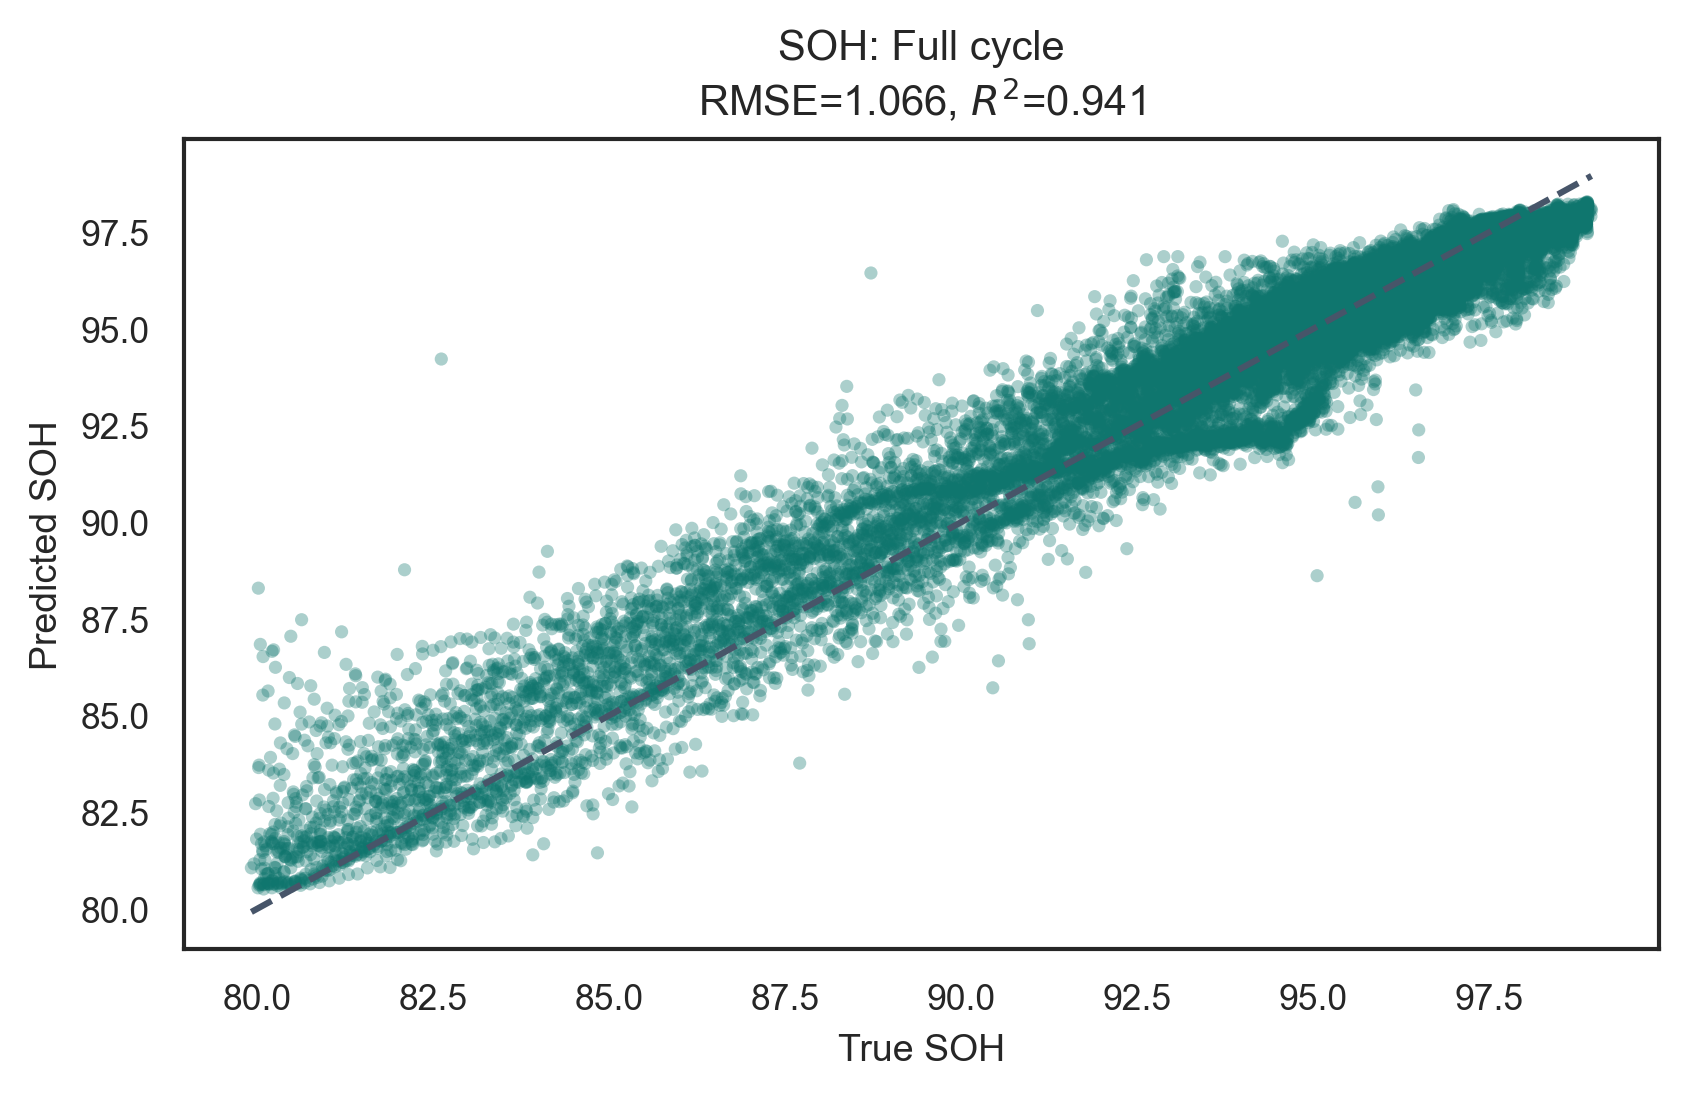
\includegraphics[width=0.8\linewidth]{../review_process/figures_revision_round1/figure_00_full_cycle_scatter_soh.png}
    \caption{Held-out prediction scatter for the baseline full-cycle \ac{soh} model.}
    \label{fig:baseline_scatter_soh_full_cycle}
\end{figure}

\begin{figure}[H]
    \centering
    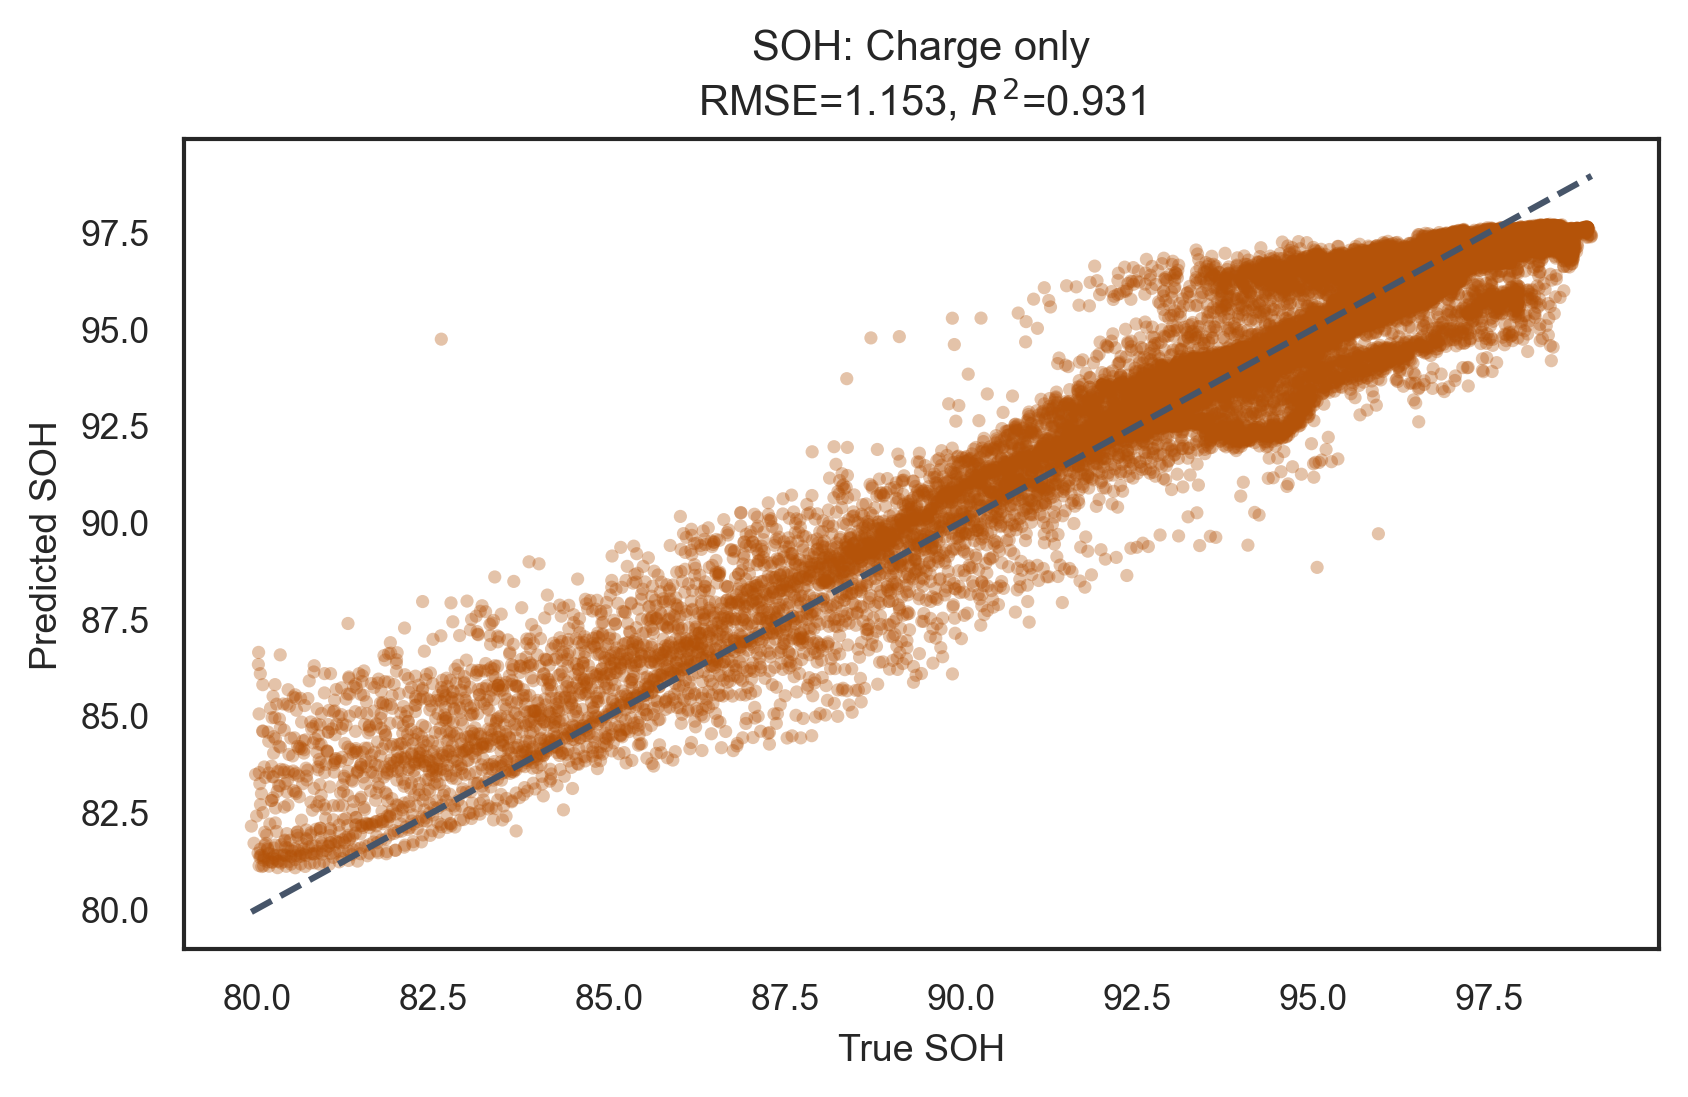
\includegraphics[width=0.8\linewidth]{../review_process/figures_revision_round1/figure_00_charge_only_scatter_soh.png}
    \caption{Held-out prediction scatter for the baseline charge-only \ac{soh} model.}
    \label{fig:baseline_scatter_soh_charge_only}
\end{figure}

\begin{figure}[H]
    \centering
    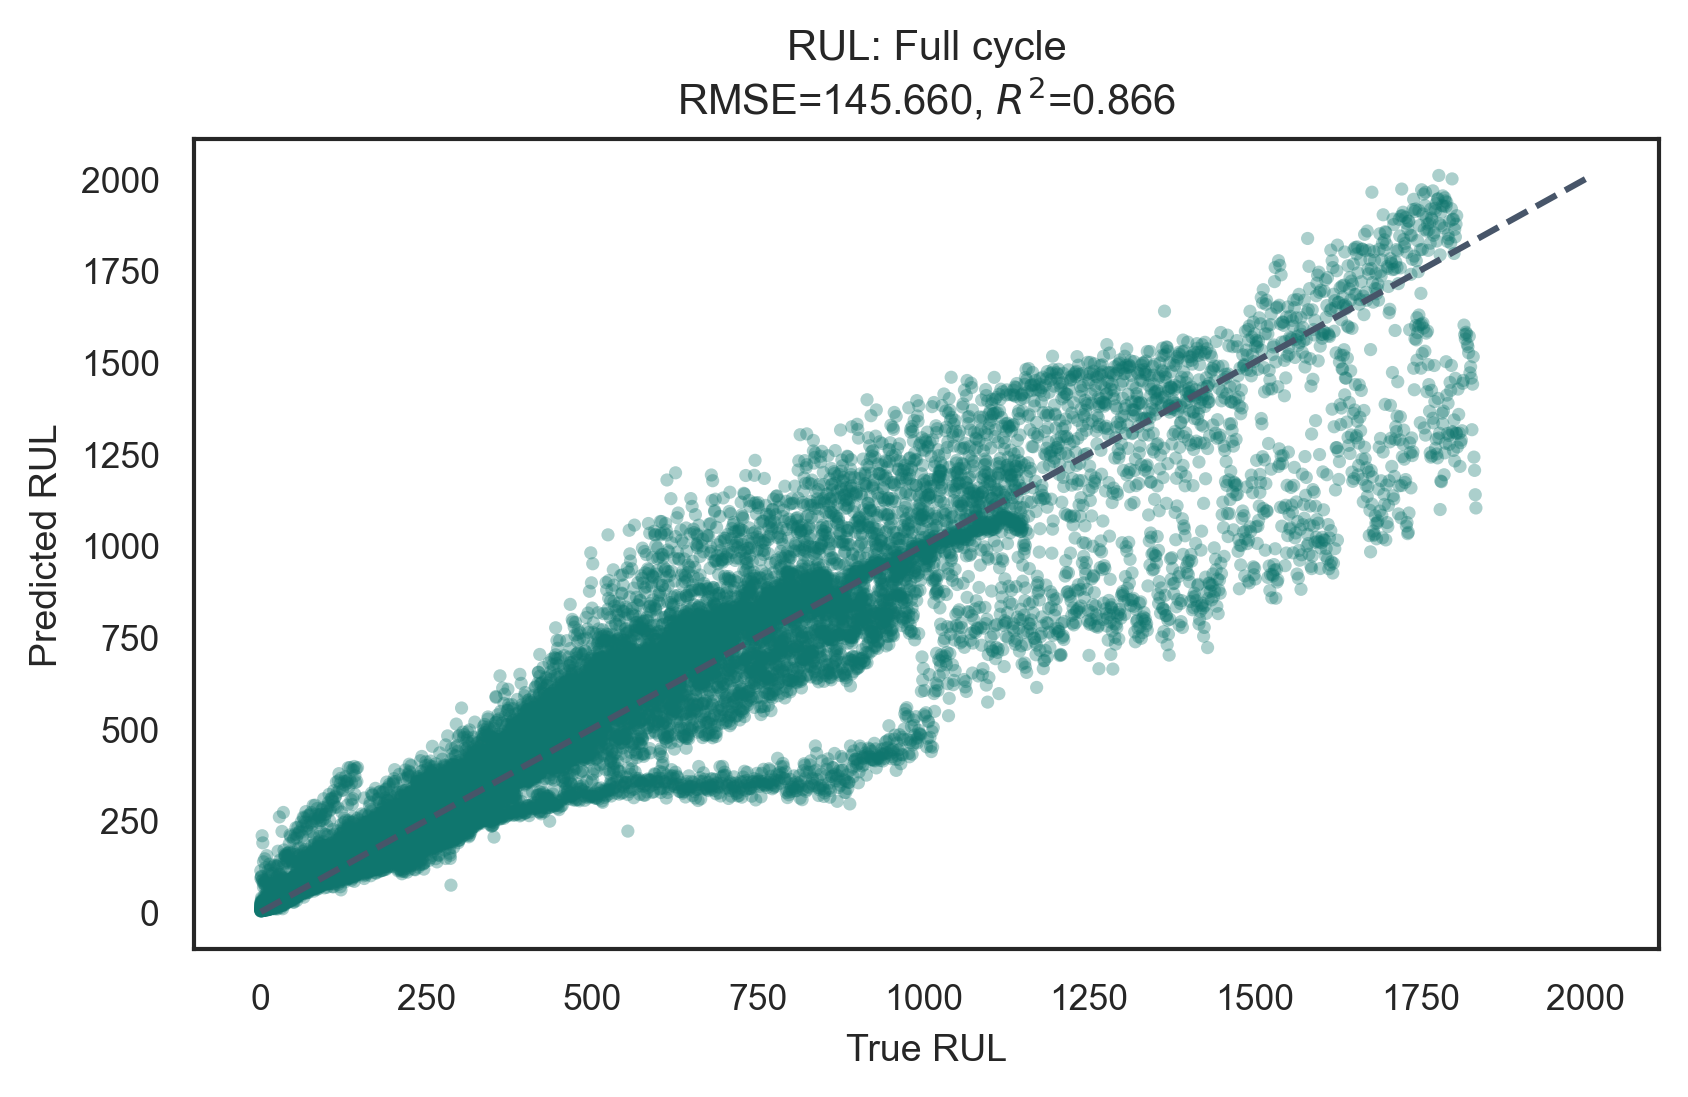
\includegraphics[width=0.8\linewidth]{../review_process/figures_revision_round1/figure_00_full_cycle_scatter_rul.png}
    \caption{Held-out prediction scatter for the baseline full-cycle \ac{rul} model.}
    \label{fig:baseline_scatter_rul_full_cycle}
\end{figure}

\begin{figure}[H]
    \centering
    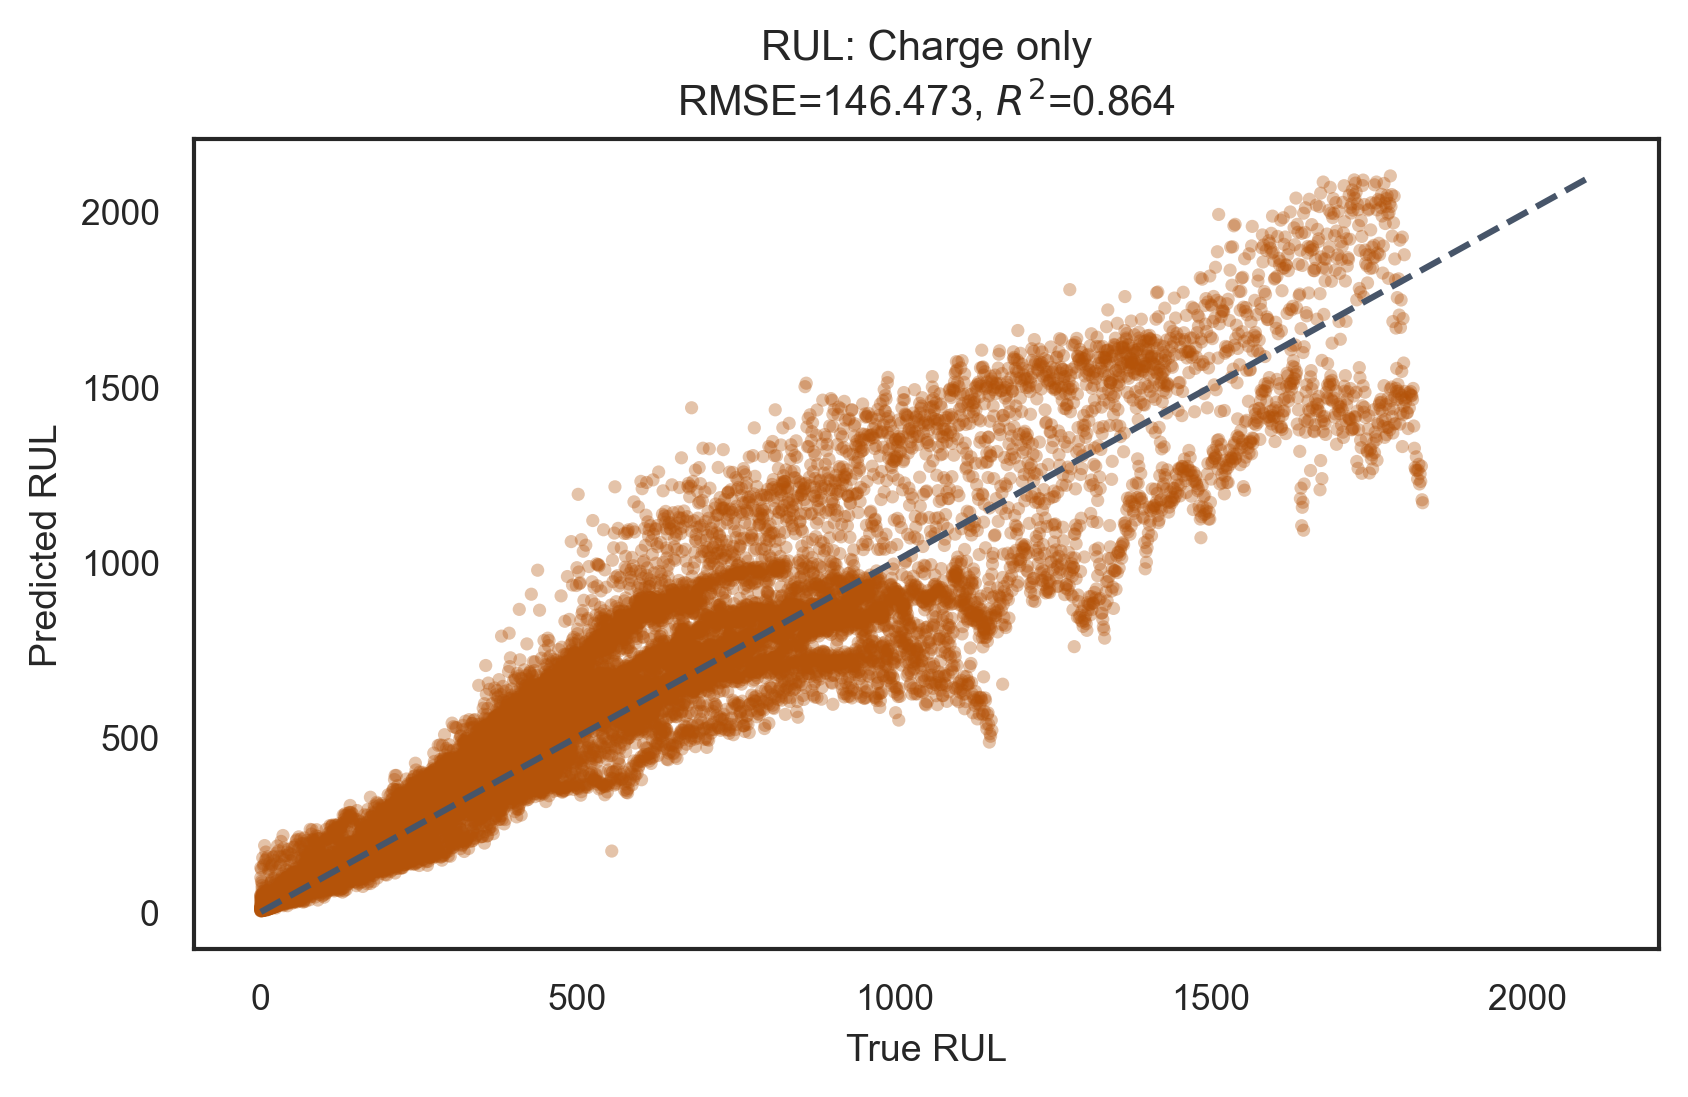
\includegraphics[width=0.8\linewidth]{../review_process/figures_revision_round1/figure_00_charge_only_scatter_rul.png}
    \caption{Held-out prediction scatter for the baseline charge-only \ac{rul} model.}
    \label{fig:baseline_scatter_rul_charge_only}
\end{figure}

\subsection{Selected Baseline Hyperparameters}

The optimized configurations are summarized in \cref{tab:baseline_hyperparams}. The \ac{rul} baselines favored deeper trees and smaller leaves than the corresponding \ac{soh} baselines, which is consistent with the higher structural complexity of lifetime prediction. The charge-only branches also indicate slightly stronger tree regularization than their full-cycle counterparts: for \ac{soh}, the charge-only model reduced \texttt{max\_depth} from 10 to 8 and \texttt{n\_estimators} from 499 to 414, while for \ac{rul} the charge-only model increased \texttt{min\_samples\_leaf} from 4 to 7 and reduced \texttt{n\_estimators} from 363 to 92.

\begin{table}[H]
    \centering
    \caption{Selected \texttt{ExtraTrees} hyperparameters for the four baseline models used in the main analyses.}
    \label{tab:baseline_hyperparams}
    \begin{tabular}{lcccc}
    \toprule
     & \multicolumn{2}{c}{\ac{soh}} & \multicolumn{2}{c}{\ac{rul}} \\
    \cmidrule(lr){2-3} \cmidrule(lr){4-5}
     & Full-cycle & Charge-only & Full-cycle & Charge-only \\
    \midrule
    \texttt{n\_estimators} & 499 & 414 & 363 & 92 \\
    \texttt{max\_depth} & 10 & 8 & 19 & 17 \\
    \texttt{min\_samples\_split} & 10 & 3 & 14 & 8 \\
    \texttt{min\_samples\_leaf} & 9 & 7 & 4 & 7 \\
    % \texttt{max\_features} & None & None & None & None \\
    \bottomrule
    \end{tabular}
\end{table}

\subsection{Feature Relevance and Compactness}

The experiments extend the baseline evaluation by explicitly analyzing which features drive prediction quality and how aggressively the feature space can be reduced before performance deteriorates. Tables~\cref{tab:full_cycle_soh_ranking,tab:full_cycle_rul_ranking} report the full-cycle feature rankings for \ac{soh} and \ac{rul}. For the full-cycle representation, the highest-ranked \ac{soh} descriptors were \(V_{\mathrm{entropy}}\), \(V_{\mathrm{std}}\), \(I_{\mathrm{iqr}}\), and \(V_{\mathrm{iqr}}\), while \ac{rul} was led by \(V_{\mathrm{iqr}}\), \(I_{\mathrm{std}}\), \(V_{\mathrm{entropy}}\), and \(V_{\mathrm{std}}\). In both cases, voltage-distribution descriptors dominate the ranking, which indicates that the prognostic information is primarily carried by the occupancy and spread of the voltage trajectory, with current statistics contributing complementary structure.

\begin{table}[H]
    \centering
    \caption{Full-cycle feature ranking summary for \ac{soh}. The ranking is based on the mean increase in validation \ac{rmse} produced by feature permutation across grouped folds and seeds.}
    \label{tab:full_cycle_soh_ranking}
    \begin{tabular}{rllr}
    \toprule
    Rank & Feature & Mean RMSE increase & Stability std \\
    \midrule
    1 & $V_{\mathrm{entropy}}$ & 1.8799 & 0.1338 \\
    2 & $V_{\mathrm{std}}$ & 0.7130 & 0.2623 \\
    3 & $I_{\mathrm{iqr}}$ & 0.4884 & 0.0473 \\
    4 & $V_{\mathrm{iqr}}$ & 0.4813 & 0.0941 \\
    5 & $I_{\mathrm{kurtosis}}$ & 0.4787 & 0.0817 \\
    6 & $V_{\mathrm{median}}$ & 0.4205 & 0.0594 \\
    7 & $I_{\mathrm{median}}$ & 0.1869 & 0.0407 \\
    8 & $I_{\mathrm{std}}$ & 0.1394 & 0.0318 \\
    9 & $V_{\mathrm{kurtosis}}$ & 0.1264 & 0.0383 \\
    10 & $I_{\mathrm{mean}}$ & 0.0814 & 0.0341 \\
    11 & $V_{\mathrm{mean}}$ & 0.0656 & 0.0255 \\
    12 & $T_{\mathrm{kurtosis}}$ & 0.0307 & 0.0082 \\
    13 & $T_{\mathrm{median}}$ & 0.0248 & 0.0117 \\
    14 & $T_{\mathrm{mean}}$ & 0.0149 & 0.0095 \\
    15 & $T_{\mathrm{iqr}}$ & 0.0006 & 0.0120 \\
    16 & $T_{\mathrm{std}}$ & -0.0026 & 0.0115 \\
    \bottomrule
    \end{tabular}
\end{table}

\begin{table}[H]
    \centering
    \caption{Full-cycle feature ranking summary for \ac{rul}. The ranking is based on the mean increase in validation \ac{rmse} produced by feature permutation across grouped folds and seeds.}
    \label{tab:full_cycle_rul_ranking}
    \begin{tabular}{rllr}
    \toprule
    Rank & Feature & Mean RMSE increase & Stability std \\
    \midrule
    1 & $V_{\mathrm{iqr}}$ & 104.4589 & 26.7059 \\
    2 & $I_{\mathrm{std}}$ & 61.3457 & 45.1326 \\
    3 & $V_{\mathrm{entropy}}$ & 48.4977 & 10.9364 \\
    4 & $V_{\mathrm{std}}$ & 47.0014 & 17.9436 \\
    5 & $I_{\mathrm{mean}}$ & 41.4087 & 9.3307 \\
    6 & $I_{\mathrm{median}}$ & 38.2823 & 20.5138 \\
    7 & $V_{\mathrm{kurtosis}}$ & 26.0695 & 5.8031 \\
    8 & $I_{\mathrm{kurtosis}}$ & 13.7206 & 6.5764 \\
    9 & $V_{\mathrm{median}}$ & 10.0335 & 2.9792 \\
    10 & $I_{\mathrm{iqr}}$ & 4.1394 & 2.1203 \\
    11 & $V_{\mathrm{mean}}$ & 4.0592 & 1.6338 \\
    12 & $T_{\mathrm{std}}$ & 3.8050 & 7.2698 \\
    13 & $T_{\mathrm{kurtosis}}$ & 3.1329 & 1.5723 \\
    14 & $T_{\mathrm{median}}$ & 1.4827 & 3.1298 \\
    15 & $T_{\mathrm{mean}}$ & 1.4340 & 2.8267 \\
    16 & $T_{\mathrm{iqr}}$ & 0.2363 & 4.9880 \\
    \bottomrule
    \end{tabular}
\end{table}

The top-\(k\) sweeps also showed that the 16-feature representation is redundant. Figures~\cref{fig:full_cycle_topk_soh,fig:full_cycle_topk_rul} show that, for full-cycle \ac{soh}, the best grouped-validation performance was observed around 10--12 features, and that the selected 6-feature subset remained within the predefined 10\% tolerance of the baseline. For full-cycle \ac{rul}, performance also peaked around 10 features, while the 6-feature subset was nearly indistinguishable from the 16-feature baseline in cross-validation. The selected full-cycle compact subsets were \(\{V_{\mathrm{entropy}}, V_{\mathrm{std}}, I_{\mathrm{iqr}}, V_{\mathrm{iqr}}, I_{\mathrm{kurtosis}}, V_{\mathrm{median}}\}\) for \ac{soh} and \(\{V_{\mathrm{iqr}}, I_{\mathrm{std}}, V_{\mathrm{entropy}}, V_{\mathrm{std}}, I_{\mathrm{mean}}, I_{\mathrm{median}}\}\) for \ac{rul}.

\begin{figure}[H]
    \centering
    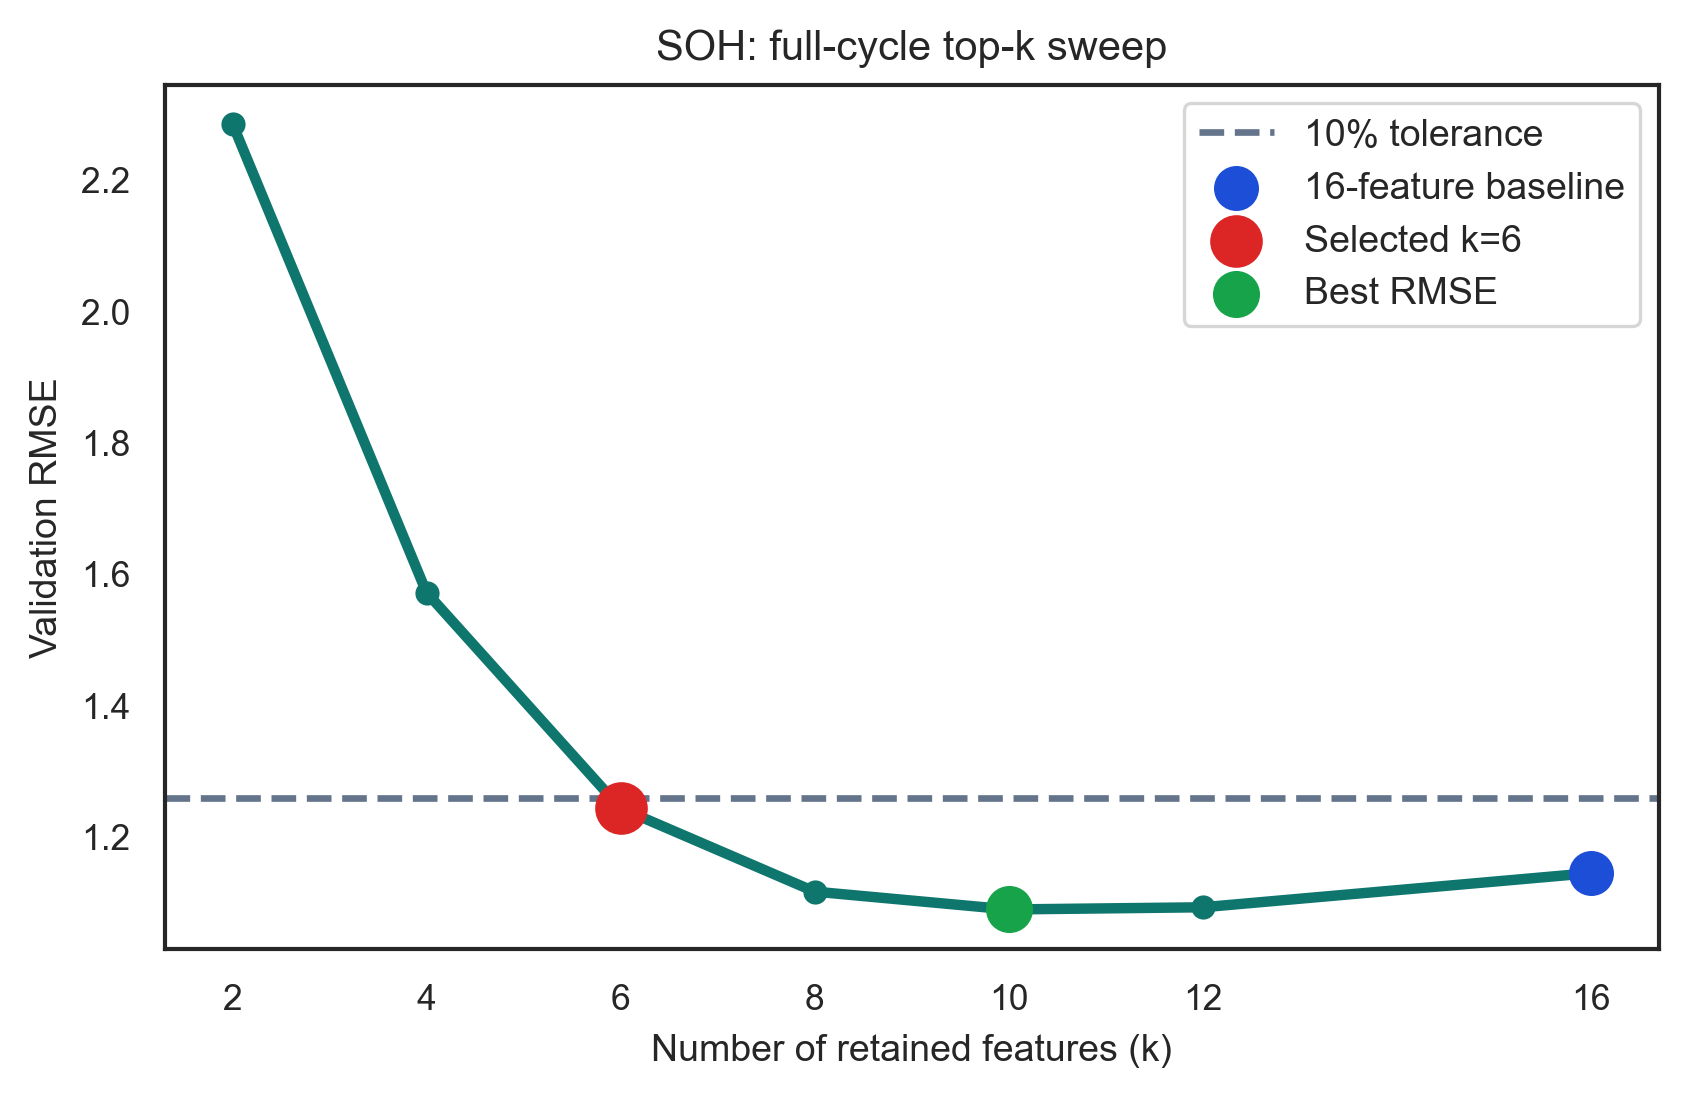
\includegraphics[width=0.8\linewidth]{../review_process/figures_revision_round1/figure_01_full_cycle_topk_soh.png}
    \caption{Top-\(k\) validation performance for the full-cycle \ac{soh} representation. The curve shows the effect of progressively reducing the ranked feature set.}
    \label{fig:full_cycle_topk_soh}
\end{figure}

\begin{figure}[H]
    \centering
    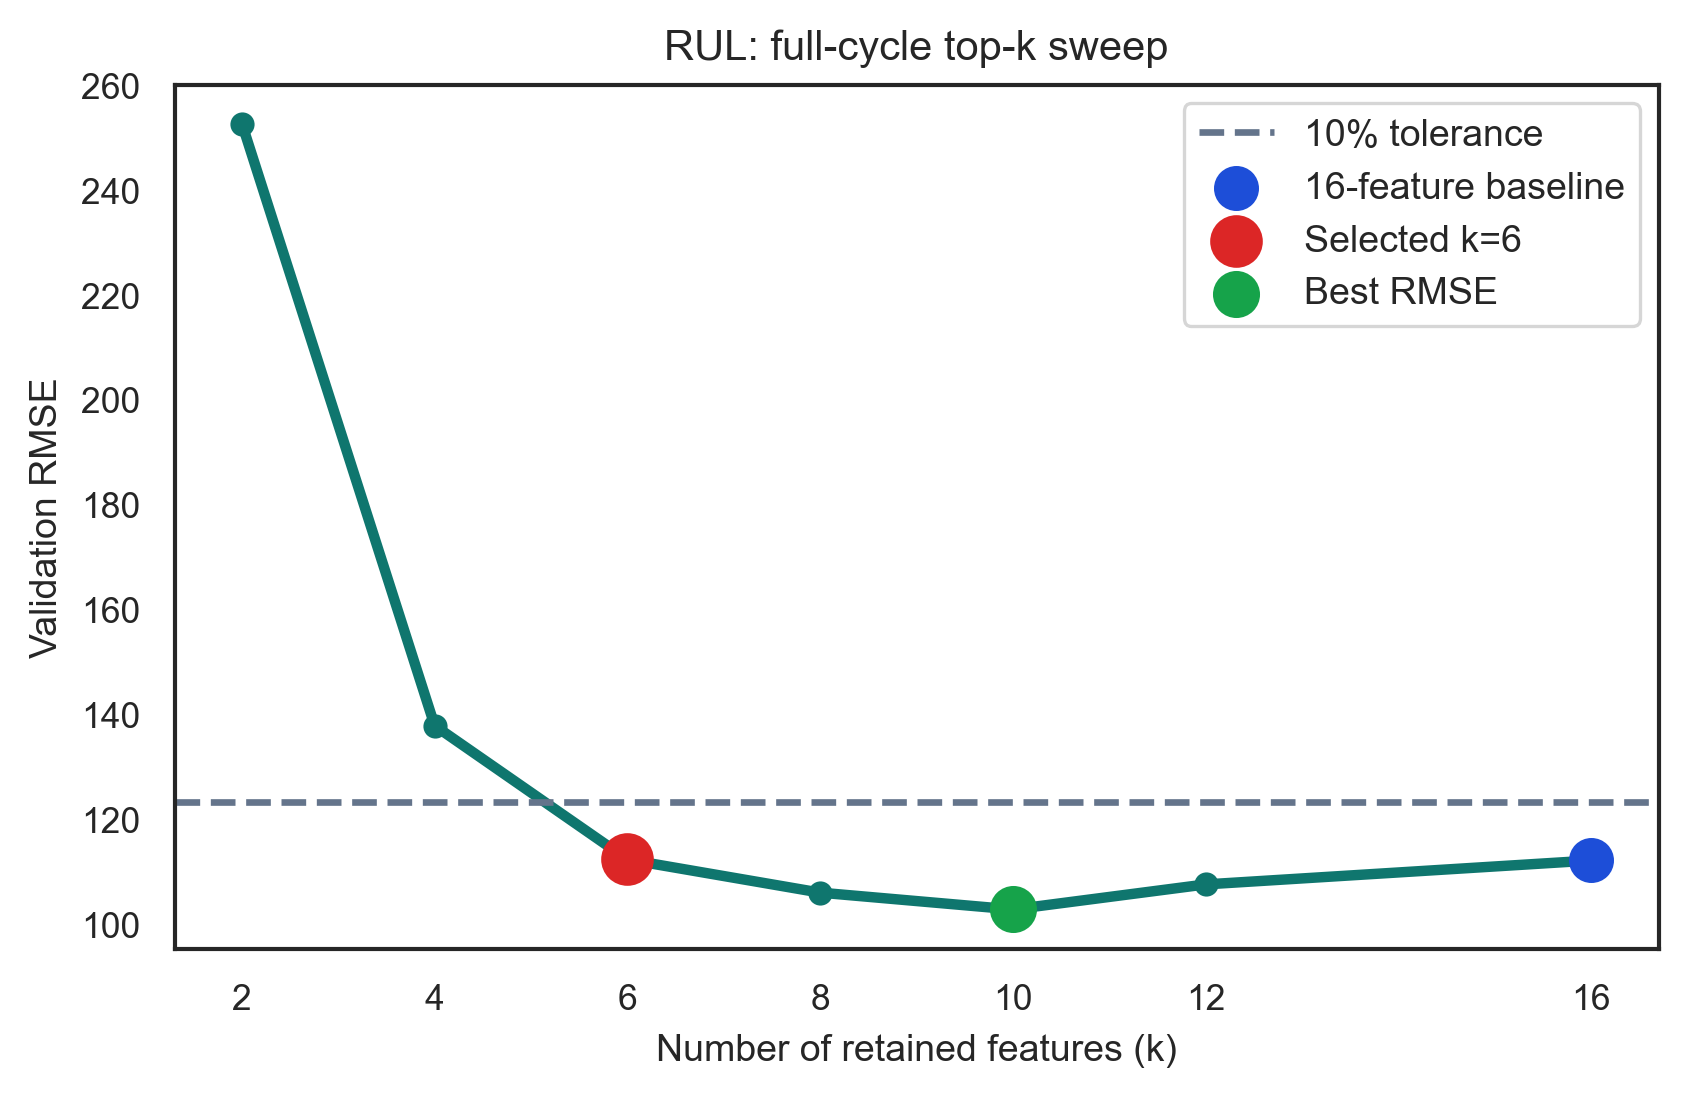
\includegraphics[width=0.8\linewidth]{../review_process/figures_revision_round1/figure_01_full_cycle_topk_rul.png}
    \caption{Top-\(k\) validation performance for the full-cycle \ac{rul} representation. The best validation region occurs at intermediate subset sizes, while the selected compact subset remains close to the full baseline.}
    \label{fig:full_cycle_topk_rul}
\end{figure}

The charge-only analyses preserved the same qualitative hierarchy, but with a more compact dominant core centered on voltage median, current median, voltage entropy, and spread statistics. Tables~\cref{tab:charge_only_soh_ranking,tab:charge_only_rul_ranking} show that this dominant core remains visible for both targets in the charge-only representation. The selected compact subsets were \(\{V_{\mathrm{median}}^{\mathrm{ch}}, I_{\mathrm{median}}^{\mathrm{ch}}, V_{\mathrm{entropy}}^{\mathrm{ch}}, V_{\mathrm{std}}^{\mathrm{ch}}, V_{\mathrm{iqr}}^{\mathrm{ch}}, I_{\mathrm{std}}^{\mathrm{ch}}\}\) for \ac{soh} and \(\{V_{\mathrm{median}}^{\mathrm{ch}}, I_{\mathrm{median}}^{\mathrm{ch}}, V_{\mathrm{entropy}}^{\mathrm{ch}}, I_{\mathrm{std}}^{\mathrm{ch}}\}\) for \ac{rul}, where the superscript \(\mathrm{ch}\) denotes features extracted from the charge segment only. These subsets should be interpreted as deployable approximations rather than strict replacements for the 16-feature baselines, since the held-out comparisons generally favored the full feature sets.

\begin{table}[H]
    \centering
    \caption{Charge-only feature ranking summary for \ac{soh}. The ranking is based on the mean increase in validation \ac{rmse} produced by feature permutation across grouped folds and seeds.}
    \label{tab:charge_only_soh_ranking}
    \begin{tabular}{rllr}
    \toprule
    Rank & Feature & Mean RMSE increase & Stability std \\
    \midrule
    1 & $V_{\mathrm{median}}^{\mathrm{ch}}$ & 1.4980 & 0.2744 \\
    2 & $I_{\mathrm{median}}^{\mathrm{ch}}$ & 1.3504 & 0.1144 \\
    3 & $V_{\mathrm{entropy}}^{\mathrm{ch}}$ & 0.9521 & 0.2044 \\
    4 & $V_{\mathrm{std}}^{\mathrm{ch}}$ & 0.5725 & 0.1228 \\
    5 & $V_{\mathrm{iqr}}^{\mathrm{ch}}$ & 0.1956 & 0.0317 \\
    6 & $I_{\mathrm{std}}^{\mathrm{ch}}$ & 0.1494 & 0.0550 \\
    7 & $I_{\mathrm{kurtosis}}^{\mathrm{ch}}$ & 0.1468 & 0.0265 \\
    8 & $V_{\mathrm{mean}}^{\mathrm{ch}}$ & 0.1049 & 0.0364 \\
    9 & $T_{\mathrm{median}}^{\mathrm{ch}}$ & 0.0865 & 0.0369 \\
    10 & $I_{\mathrm{iqr}}^{\mathrm{ch}}$ & 0.0709 & 0.0134 \\
    11 & $I_{\mathrm{mean}}^{\mathrm{ch}}$ & 0.0611 & 0.0153 \\
    12 & $V_{\mathrm{kurtosis}}^{\mathrm{ch}}$ & 0.0464 & 0.0300 \\
    13 & $T_{\mathrm{kurtosis}}^{\mathrm{ch}}$ & 0.0322 & 0.0105 \\
    14 & $T_{\mathrm{mean}}^{\mathrm{ch}}$ & 0.0243 & 0.0072 \\
    15 & $T_{\mathrm{iqr}}^{\mathrm{ch}}$ & 0.0144 & 0.0144 \\
    16 & $T_{\mathrm{std}}^{\mathrm{ch}}$ & 0.0054 & 0.0058 \\
    \bottomrule
    \end{tabular}
\end{table}

\begin{table}[H]
    \centering
    \caption{Charge-only feature ranking summary for \ac{rul}. The ranking is based on the mean increase in validation \ac{rmse} produced by feature permutation across grouped folds and seeds.}
    \label{tab:charge_only_rul_ranking}
    \begin{tabular}{rllr}
    \toprule
    Rank & Feature & Mean RMSE increase & Stability std \\
    \midrule
    1 & $V_{\mathrm{median}}^{\mathrm{ch}}$ & 213.8374 & 32.8777 \\
    2 & $I_{\mathrm{median}}^{\mathrm{ch}}$ & 68.0544 & 27.7644 \\
    3 & $V_{\mathrm{entropy}}^{\mathrm{ch}}$ & 32.4691 & 14.7522 \\
    4 & $I_{\mathrm{std}}^{\mathrm{ch}}$ & 31.4898 & 34.7147 \\
    5 & $V_{\mathrm{iqr}}^{\mathrm{ch}}$ & 21.5297 & 6.6023 \\
    6 & $I_{\mathrm{mean}}^{\mathrm{ch}}$ & 14.1291 & 15.9031 \\
    7 & $V_{\mathrm{mean}}^{\mathrm{ch}}$ & 5.5687 & 6.6184 \\
    8 & $I_{\mathrm{kurtosis}}^{\mathrm{ch}}$ & 5.3358 & 11.4103 \\
    9 & $V_{\mathrm{std}}^{\mathrm{ch}}$ & 4.8521 & 3.0310 \\
    10 & $T_{\mathrm{median}}^{\mathrm{ch}}$ & 2.5104 & 3.5594 \\
    11 & $T_{\mathrm{kurtosis}}^{\mathrm{ch}}$ & 2.2075 & 2.6434 \\
    12 & $T_{\mathrm{mean}}^{\mathrm{ch}}$ & 1.8858 & 3.4237 \\
    13 & $I_{\mathrm{iqr}}^{\mathrm{ch}}$ & 1.7905 & 4.2008 \\
    14 & $V_{\mathrm{kurtosis}}^{\mathrm{ch}}$ & 1.6188 & 1.6187 \\
    15 & $T_{\mathrm{iqr}}^{\mathrm{ch}}$ & -2.1075 & 4.2539 \\
    16 & $T_{\mathrm{std}}^{\mathrm{ch}}$ & -3.1912 & 7.7093 \\
    \bottomrule
    \end{tabular}
\end{table}

\begin{figure}[H]
    \centering
    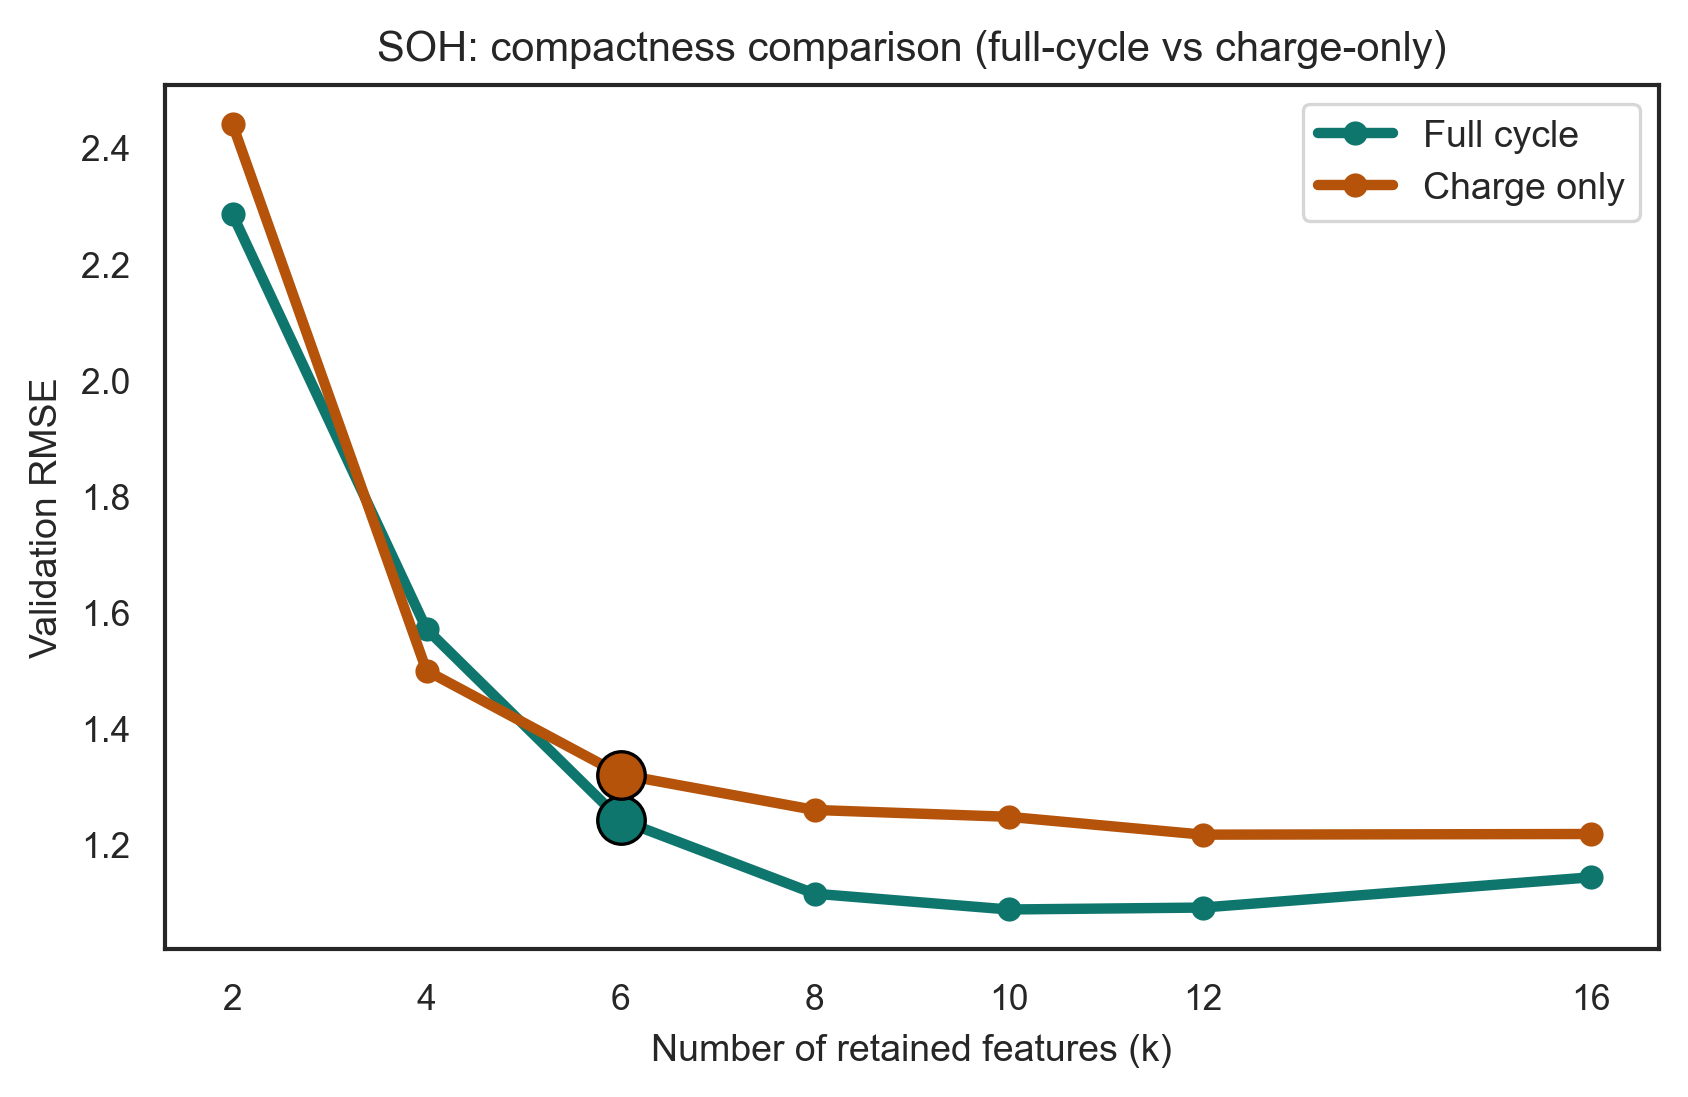
\includegraphics[width=0.8\linewidth]{../review_process/figures_revision_round1/figure_02_compactness_comparison_soh.png}
    \caption{Compactness comparison for \ac{soh}. Full-cycle and charge-only feature subsets show the trade-off between representation size and validation error.}
    \label{fig:compactness_comparison_soh}
\end{figure}

\begin{figure}[H]
    \centering
    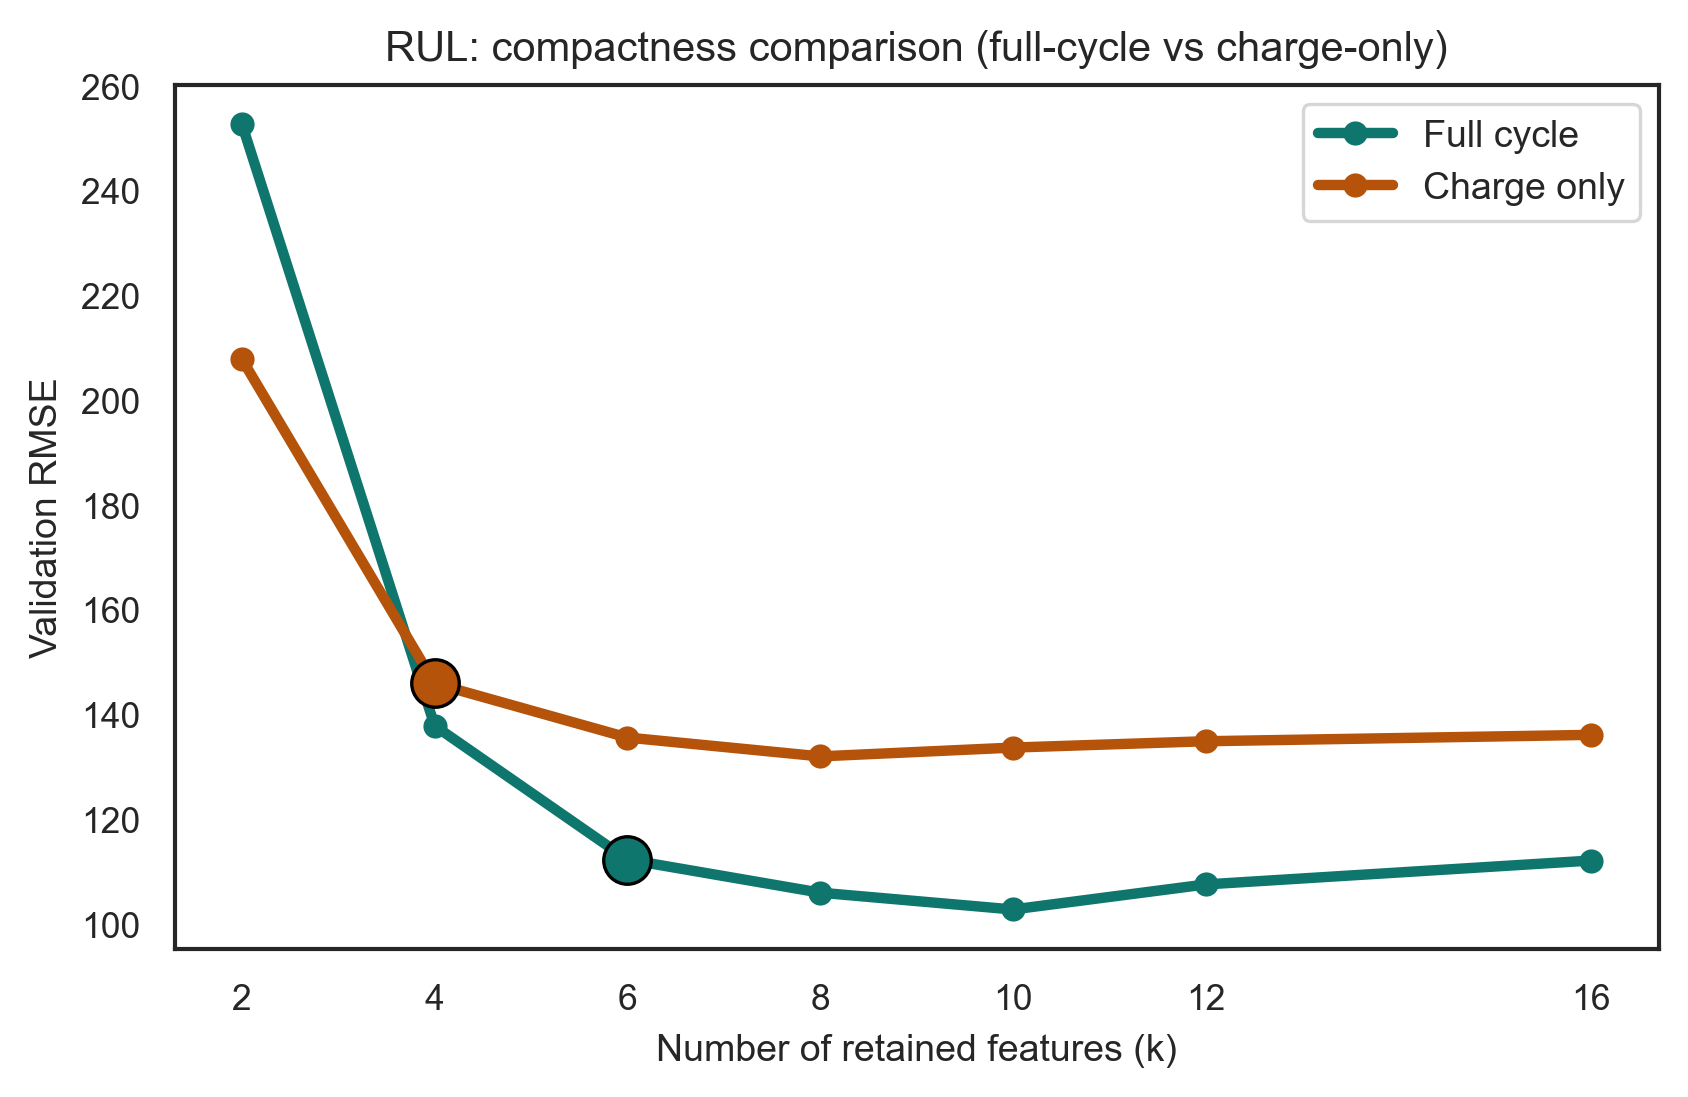
\includegraphics[width=0.8\linewidth]{../review_process/figures_revision_round1/figure_02_compactness_comparison_rul.png}
    \caption{Compactness comparison for \ac{rul}. The charge-only representation is more sensitive to aggressive reduction, but both views retain useful prognostic information at compact subset sizes.}
    \label{fig:compactness_comparison_rul}
\end{figure}

\begin{table}[H]
    \centering
    \caption{Compact-subset results. The grouped-validation columns correspond to the selected top-\(k\) subset in each branch, while the test columns summarize the held-out evaluations performed after subset selection.}
    \label{tab:compact_subset_summary_transposed}
    \begin{tabular}{lcccc}
    \toprule
     & \multicolumn{2}{c}{\ac{soh}} & \multicolumn{2}{c}{\ac{rul}} \\
    \cmidrule(lr){2-3} \cmidrule(lr){4-5}
     & Full-cycle & Charge-only & Full-cycle & Charge-only \\
    \midrule
    Features & 6 & 6 & 6 & 4 \\
    Val. RMSE & 1.2422 & 1.3203 & 112.2295 & 145.8439 \\
    Test RMSE & 1.2474 & 1.2999 & 156.6287 & 151.4424 \\
    Test $R^2$ & 0.9191 & 0.9121 & 0.8450 & 0.8551 \\
    \bottomrule
    \end{tabular}
\end{table}

The compactness trade-off is summarized visually in \cref{fig:compactness_comparison_soh,fig:compactness_comparison_rul} and numerically in \cref{tab:compact_subset_summary_transposed}. Taken together, these results support two practical claims. First, most of the predictive value is concentrated in a small subset of voltage-current descriptors. Second, the compact models are credible when deployment simplicity matters, but the original 16-feature baselines remain the strongest reference points for the main held-out comparisons.

\subsection{Temperature Ablation}

Another consistent result is the weak and unstable marginal contribution of temperature-derived statistics. Table~\cref{tab:no_temperature_summary_transposed} reports the corresponding ablation results. In the grouped-validation ablations, removing all temperature features improved the full-cycle baselines for both targets and improved the charge-only baseline for \ac{rul}, while remaining nearly neutral for charge-only \ac{soh}. The held-out results were more asymmetric: no-temperature full-cycle \ac{soh} improved slightly over the original baseline, full-cycle \ac{rul} degraded, charge-only \ac{soh} changed only marginally, and charge-only \ac{rul} improved substantially.

\begin{table}[H]
    \centering
    \caption{No-temperature results. Baseline test values are included to show the held-out impact of removing temperature-derived statistics.}
    \label{tab:no_temperature_summary_transposed}
    \begin{tabular}{lcccc}
    \toprule
     & \multicolumn{2}{c}{\ac{soh}} & \multicolumn{2}{c}{\ac{rul}} \\
    \cmidrule(lr){2-3} \cmidrule(lr){4-5}
     & Full-cycle & Charge-only & Full-cycle & Charge-only \\
    \midrule
    Baseline test RMSE & 1.0660 & 1.1532 & 145.6603 & 146.4735 \\
    No-temp test RMSE & 1.0243 & 1.1627 & 153.3099 & 128.5170 \\
    Baseline test $R^2$ & 0.9409 & 0.9308 & 0.8660 & 0.8645 \\
    No-temp test $R^2$ & 0.9454 & 0.9297 & 0.8515 & 0.8956 \\
    \bottomrule
    \end{tabular}
\end{table}

These ablations do not support the strong claim that temperature is uniformly harmful, but they do indicate that voltage-current statistics form the more stable prognostic core in this dataset. This point is relevant for deployment because temperature measurements are often noisier and harder to standardize than voltage and current under both laboratory and field conditions.

\subsection{Repeated-Seed Stability}
\label{sec:results_seed_stability}

This analysis starts from the best full-cycle \texttt{ExtraTrees} baseline and keeps the same optimized hyperparameters reported in \cref{tab:baseline_hyperparams}. Instead of refitting the model on cross-validation folds, the uncertainty analysis retrains the model 20 times on the full training partition using different random seeds and evaluates all repeated predictions on the same held-out test cells. The purpose is to quantify seed-induced prediction variability under the final deployment-oriented training setting, while preserving the same statistical feature representation used in the baseline full-cycle models.

To interpret this variability along the degradation trajectory, the test cycles were grouped into \ac{soh}-defined life regions using the standard 80\% end-of-life convention. Early-Life corresponds to \(95\%\leq \ac{soh}\leq 100\%\), Mid-Life to \(85\%\leq \ac{soh}<95\%\), and Aged to \(80\%\leq \ac{soh}<85\%\). Thus, the Aged region represents cells that are close to the end-of-life threshold but have not yet crossed it. The same region boundaries were used when summarizing both \ac{soh} and \ac{rul} uncertainty so that the two targets could be compared over a common degradation axis.

The test-set analysis complements the baseline metrics with repeated-seed uncertainty estimates and error stratification by life region. Table~\cref{tab:uncertainty_by_region} summarizes the repeated-seed metrics by region. For \ac{soh}, both predictive error and seed-induced prediction spread worsen as the cell approaches end-of-life: the mean prediction standard deviation increases from 0.0298 percentage points in the early-life region to 0.0632 in the aged region, while the corresponding \ac{rmse} rises from 0.7308 to 1.8385. For \ac{rul}, the absolute behavior is reversed because the remaining-life scale itself shrinks as the cell ages: the early-life region shows the highest error and uncertainty, whereas the aged region has the lowest absolute cycle error. The main implication is that predictive reliability is strongly stage-dependent for both targets, but not in the same way.

\begin{table}[H]
    \centering
    \caption{Repeated-seed uncertainty summary by life region. Regions were defined from \ac{soh} using the standard end-of-life convention.}
    \label{tab:uncertainty_by_region}
    \begin{tabular}{llrrrr}
    \toprule
    Target & Region & RMSE & MAE & $R^2$ & Mean pred. std \\
    \midrule
    \ac{soh} & Early-Life & 0.7308 & 0.5911 & 0.4708 & 0.0298 \\
    \ac{soh} & Mid-Life & 1.2622 & 1.0044 & 0.7941 & 0.0570 \\
    \ac{soh} & Aged & 1.8385 & 1.3771 & -0.6453 & 0.0632 \\
    \ac{rul} & Early-Life & 162.7012 & 105.2180 & 0.8291 & 6.1061 \\
    \ac{rul} & Mid-Life & 134.4387 & 80.5313 & 0.7090 & 4.3451 \\
    \ac{rul} & Aged & 34.3064 & 19.4232 & -0.2420 & 1.2629 \\
    \bottomrule
    \end{tabular}
\end{table}

This regional behavior is consistent with the training support available in the dataset. The aged \ac{soh} region contains far fewer samples than the early- and mid-life regions, which likely contributes to the observed deterioration. This pattern is also visible in the repeated-seed scatter plots of \cref{fig:uncertainty_scatter_soh,fig:uncertainty_scatter_rul}, where the dispersion changes systematically across life regions. The results therefore suggest that part of the late-life difficulty is methodological and part is statistical, arising from reduced support in the most degraded range.

\begin{figure}[H]
    \centering
    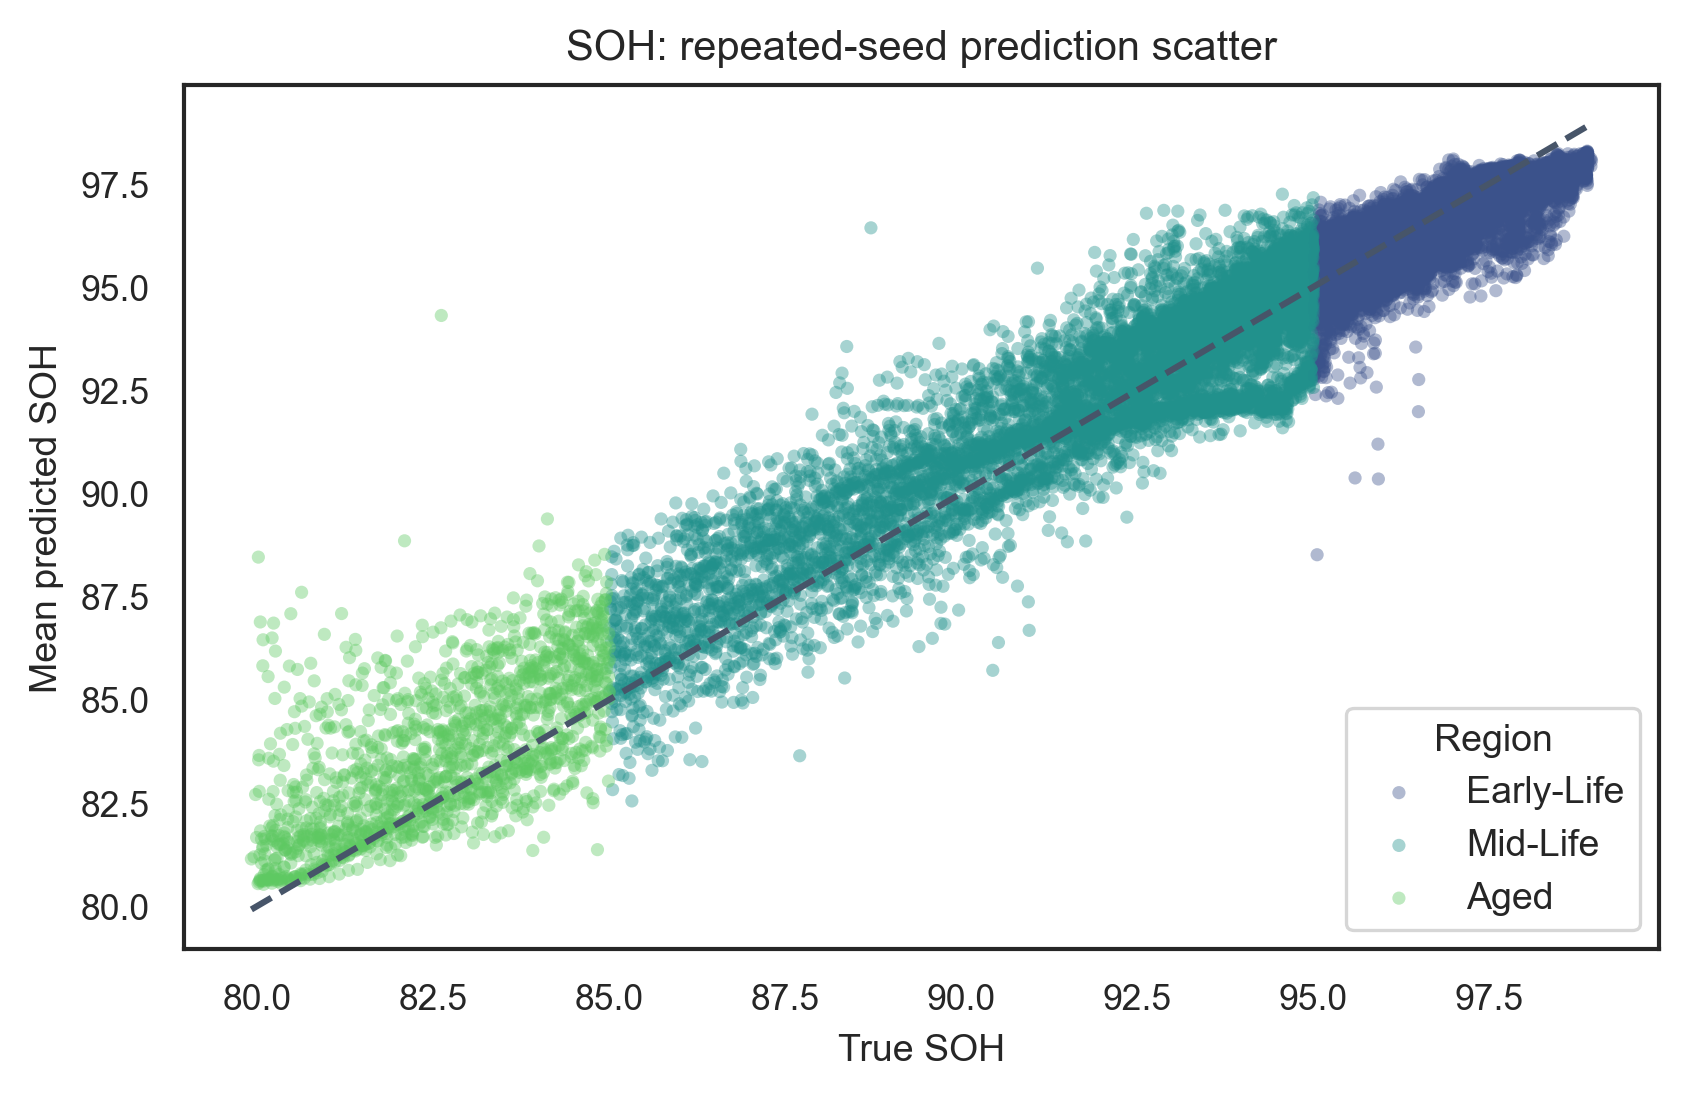
\includegraphics[width=0.8\linewidth]{../review_process/figures_revision_round1/figure_03_uncertainty_scatter_soh.png}
    \caption{Repeated-seed prediction scatter for \ac{soh}. Points are grouped by life region, and the plotted prediction corresponds to the mean over repeated retraining runs using different random seeds.}
    \label{fig:uncertainty_scatter_soh}
\end{figure}

\begin{figure}[H]
    \centering
    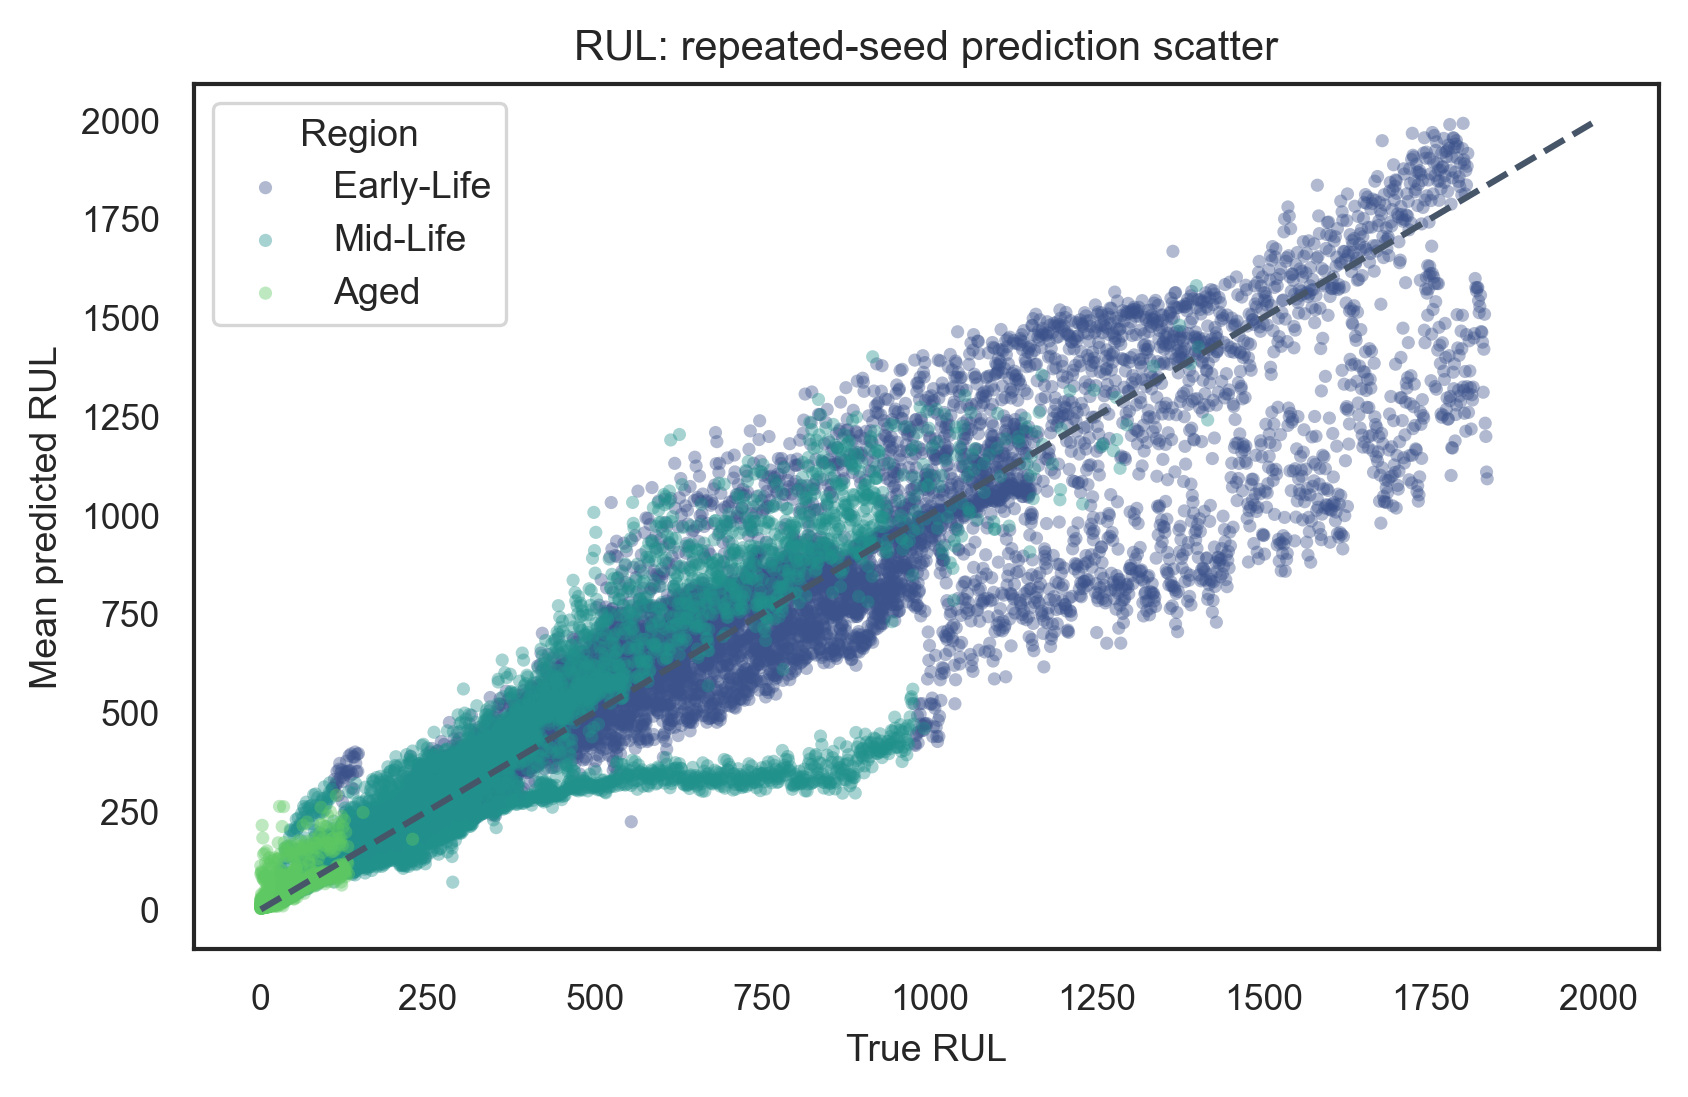
\includegraphics[width=0.8\linewidth]{../review_process/figures_revision_round1/figure_03_uncertainty_scatter_rul.png}
    \caption{Repeated-seed prediction scatter for \ac{rul}. The region coloring follows the \ac{soh}-based life partition used in the uncertainty analysis.}
    \label{fig:uncertainty_scatter_rul}
\end{figure}

\subsection{Individual Cell Diagnostics}
\label{sec:results_cell_diagnostics}

This diagnostic analysis was performed for the full-cycle \texttt{ExtraTrees} baselines, using the same held-out predictions summarized in \cref{tab:baseline_optimization_summary}. To make the notion of difficult cells reproducible, the analysis defines the worst quartile of held-out cells separately for each target, which corresponds to the 7 cells with the largest per-cell \ac{rmse} out of the 25 test cells. The diagnostics show that held-out error is not evenly distributed across cells. Instead, a limited group contributes disproportionately to the total error, especially for \ac{rul}. Table~\cref{tab:diagnostics_filtered_summary} quantifies the change in overall performance when those worst-quartile cells are excluded. For \ac{soh}, the worst-quartile cells average 1.4404 \ac{rmse}, while the remaining cells average 0.7750, which corresponds to an 85.9\% increase. For \ac{rul}, the same split is much sharper: the worst-quartile cells average 172.64 cycles \ac{rmse}, compared with 48.92 cycles for the remaining cells, corresponding to a 252.9\% increase. This concentration indicates that the dominant weakness of the method is not uniform model failure, but sensitivity to a subset of atypical degradation trajectories.

Several cells recur across both targets, including \texttt{b3c7}, \texttt{b1c3}, \texttt{b2c1}, \texttt{b1c0}, and \texttt{b3c39}. Tables~\cref{tab:worst_cells_soh,tab:worst_cells_rul} list these worst-quartile cells and their dominant error regions. Their repeated appearance suggests that the difficult cases are structurally unusual relative to the training population rather than being target-specific accidents. For \ac{soh}, the dominant error region is often late life, whereas for \ac{rul} it is more often early or mid life, which is consistent with the stage-dependent behavior reported in \cref{sec:results_seed_stability} and with the larger absolute \ac{rul} scale far from end-of-life.

The additional cell-level inspection also helps delimit what these difficult cases are not. The five cells that appear in the worst quartile for both targets are associated with the specific protocols \texttt{3.6C(80\%)-3.6C} (\texttt{b1c0}), \texttt{4C(80\%)-4C} (\texttt{b1c3}), \texttt{2C(10\%)-6C} (\texttt{b2c1}), \texttt{4.8C(80\%)-4.8C-newstructure} (\texttt{b3c7}), and \texttt{5.3C(54\%)-4C-newstructure} (\texttt{b3c39}), which already shows that the overlap is not restricted to a single charging recipe. Their cycle lives are 1806, 1432, 146, 1834, and 1154 cycles, respectively. Relative to the training-cell distribution, whose minimum, first quartile, third quartile, and maximum cycle lives are 299, 499.5, 931.5, and 2235 cycles, \texttt{b2c1} lies below the observed training range, whereas the other four overlapping cells lie above the third quartile and two of them approach the upper tail. This indicates that the largest recurrent errors are associated less with family novelty than with cells occupying the tails of the lifetime distribution.

\begin{table}[H]
    \centering
    \caption{Held-out performance before and after excluding the worst-quartile cells identified by per-cell \ac{rmse}.}
    \label{tab:diagnostics_filtered_summary}
    \begin{tabular}{llrr}
    \toprule
    Target & Evaluation set & RMSE & $R^2$ \\
    \midrule
    \ac{soh} & All held-out cells & 1.0660 & 0.9409 \\
    \ac{soh} & Remaining 75\% of cells & 0.7852 & 0.9673 \\
    \ac{rul} & All held-out cells & 145.6603 & 0.8660 \\
    \ac{rul} & Remaining 75\% of cells & 55.4133 & 0.9526 \\
    \bottomrule
    \end{tabular}
\end{table}

\begin{figure}[H]
    \centering
    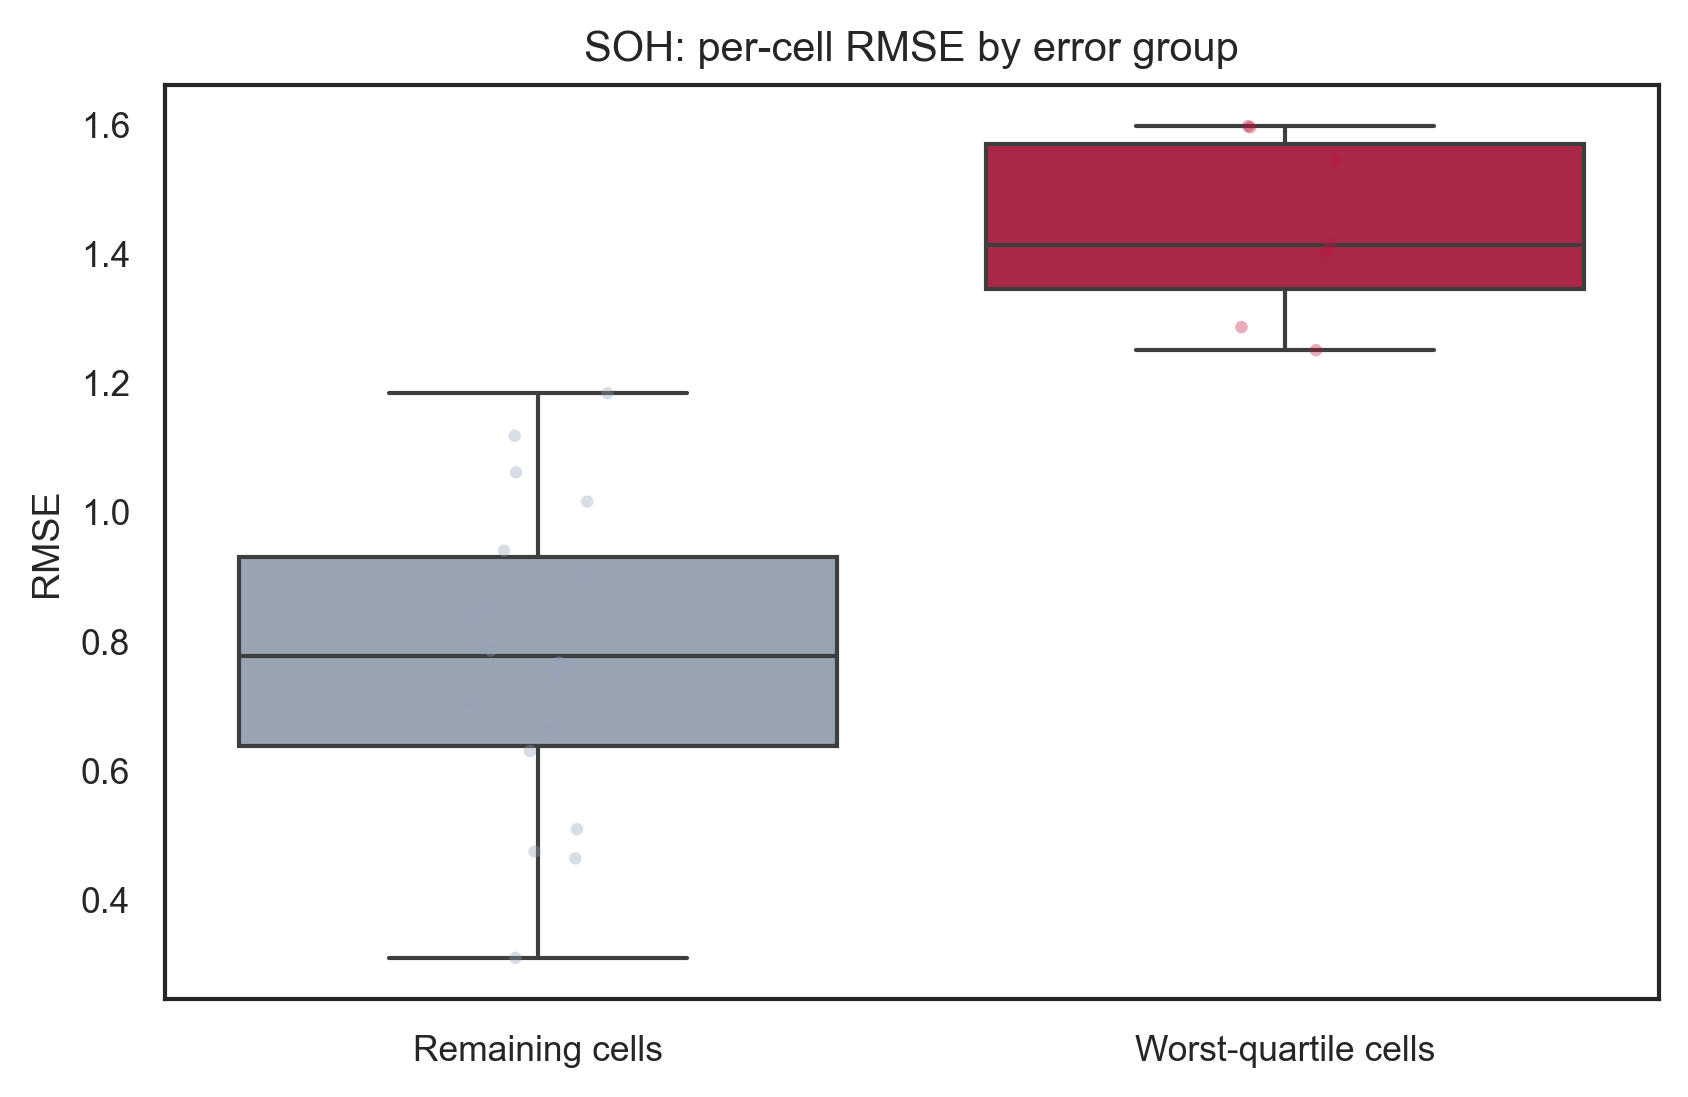
\includegraphics[width=0.8\linewidth]{../review_process/figures_revision_round1/figure_04_rmse_boxplot_soh.png}
    \caption{Per-cell \ac{rmse} distributions for the worst-quartile and remaining held-out cells in the \ac{soh} diagnostics.}
    \label{fig:diagnostics_rmse_groups_soh}
\end{figure}

\begin{figure}[H]
    \centering
    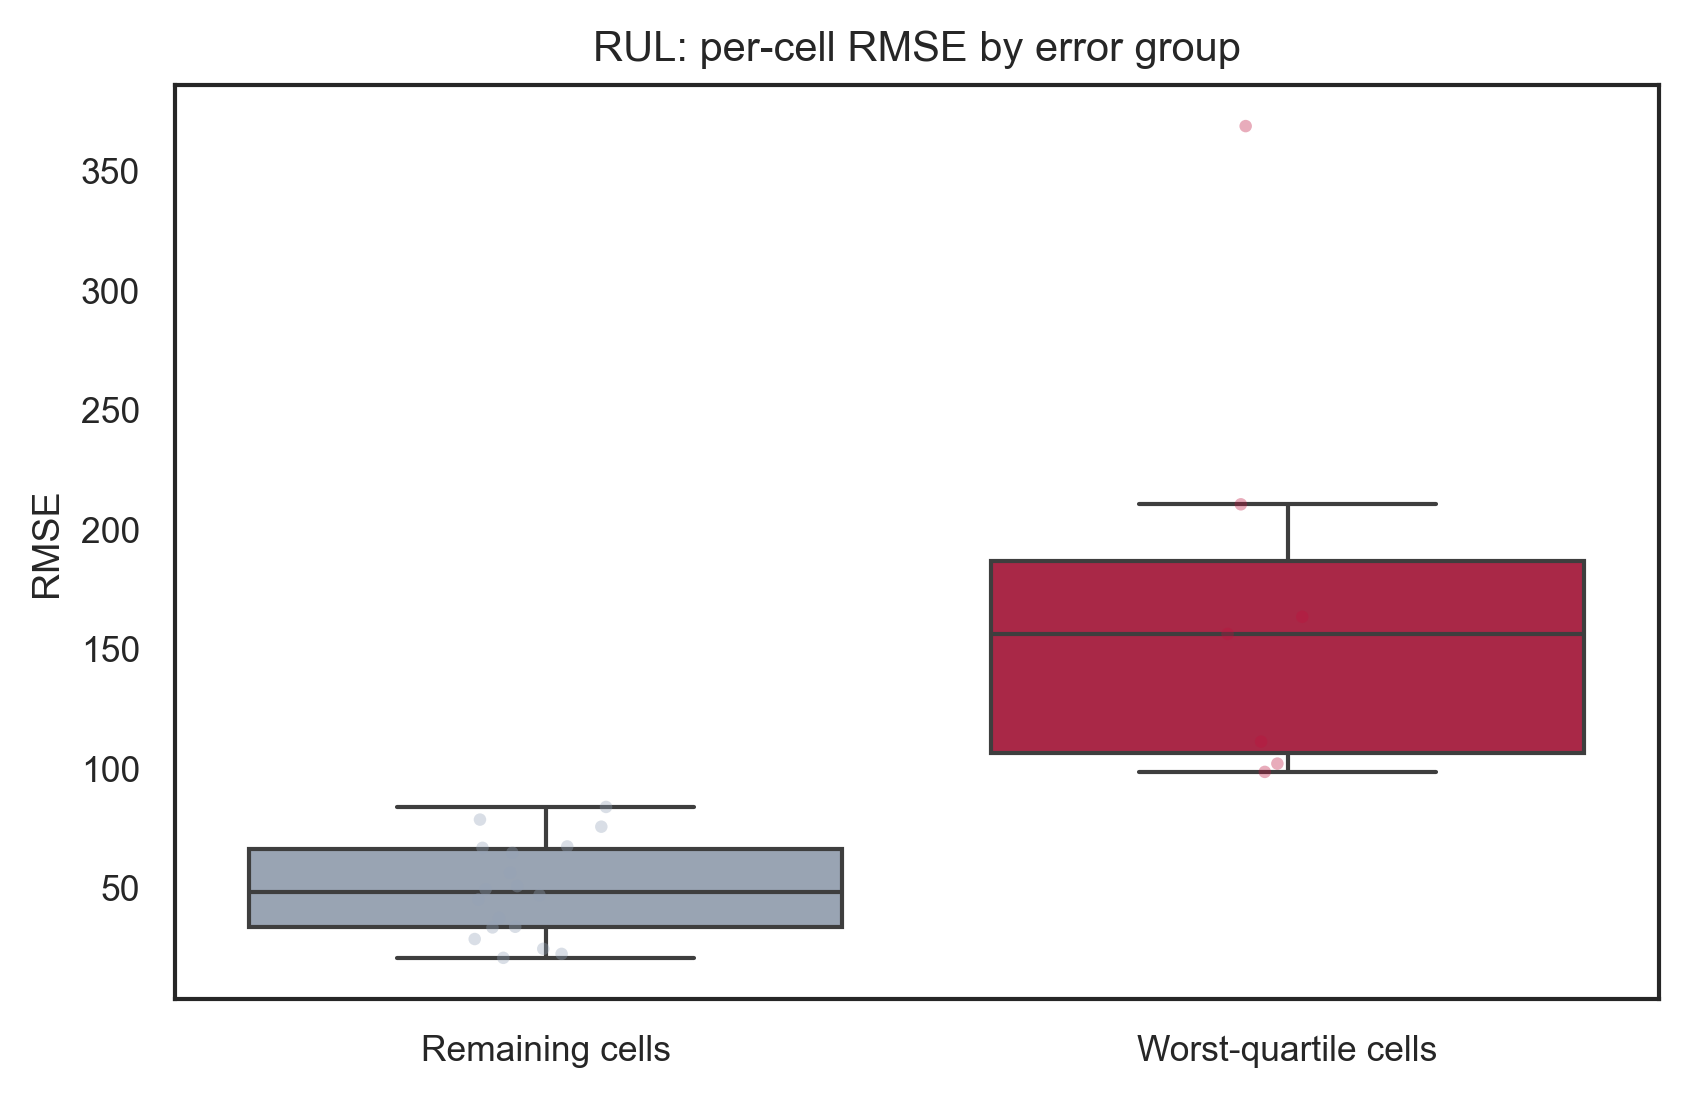
\includegraphics[width=0.8\linewidth]{../review_process/figures_revision_round1/figure_04_rmse_boxplot_rul.png}
    \caption{Per-cell \ac{rmse} distributions for the worst-quartile and remaining held-out cells in the \ac{rul} diagnostics.}
    \label{fig:diagnostics_rmse_groups_rul}
\end{figure}

\begin{table}[H]
    \centering
    \caption{Worst-quartile held-out cells for \ac{soh} in the full-cycle diagnostics. Cells that also appear in the \ac{rul} worst-quartile list are underlined.}
    \label{tab:worst_cells_soh}
    \begin{tabular}{lrrl}
    \toprule
    Cell & RMSE & $R^2$ & Dominant error region \\
    \midrule
    \texttt{b1c20} & 1.5963 & 0.8819 & late\_life \\
    \underline{\texttt{b1c0}} & 1.5944 & 0.8624 & late\_life \\
    \underline{\texttt{b2c1}} & 1.5439 & 0.9102 & late\_life \\
    \underline{\texttt{b3c7}} & 1.4120 & 0.8819 & mid\_life \\
    \texttt{b2c42} & 1.4018 & 0.9078 & late\_life \\
    \underline{\texttt{b1c3}} & 1.2853 & 0.9311 & late\_life \\
    \underline{\texttt{b3c39}} & 1.2494 & 0.8390 & late\_life \\
    \bottomrule
    \end{tabular}
\end{table}

\begin{table}[H]
    \centering
    \caption{Worst-quartile held-out cells for \ac{rul} in the full-cycle diagnostics. Cells that also appear in the \ac{soh} worst-quartile list are underlined.}
    \label{tab:worst_cells_rul}
    \begin{tabular}{lrrl}
    \toprule
    Cell & RMSE & $R^2$ & Dominant error region \\
    \midrule
    \underline{\texttt{b3c7}} & 368.4326 & 0.5162 & early\_life \\
    \underline{\texttt{b1c3}} & 210.1822 & 0.7415 & mid\_life \\
    \underline{\texttt{b2c1}} & 163.1153 & -13.7760 & early\_life \\
    \underline{\texttt{b1c0}} & 155.9591 & 0.9104 & mid\_life \\
    \texttt{b3c25} & 110.8863 & 0.8488 & early\_life \\
    \underline{\texttt{b3c39}} & 101.6881 & 0.9070 & mid\_life \\
    \texttt{b1c36} & 98.2172 & 0.7651 & mid\_life \\
    \bottomrule
    \end{tabular}
\end{table}

\begin{table}[p]
    \centering
    \caption{Per-cell held-out metrics for \ac{soh}, computed from the saved prediction artifacts.}
    \label{tab:per_cell_metrics_soh}
    \begin{tabular}{lrr}
    \toprule
    Cell & RMSE & $R^2$ \\
    \midrule
    \texttt{b1c0} & 1.5944 & 0.8624 \\
    \texttt{b1c15} & 0.8472 & 0.9579 \\
    \texttt{b1c20} & 1.5963 & 0.8819 \\
    \texttt{b1c21} & 0.8376 & 0.9641 \\
    \texttt{b1c29} & 0.6290 & 0.9814 \\
    \texttt{b1c3} & 1.2853 & 0.9311 \\
    \texttt{b1c36} & 0.9007 & 0.9614 \\
    \texttt{b1c37} & 0.7849 & 0.9685 \\
    \texttt{b1c40} & 1.0152 & 0.9530 \\
    \texttt{b1c45} & 1.1830 & 0.9427 \\
    \texttt{b2c1} & 1.5439 & 0.9102 \\
    \texttt{b2c11} & 0.7501 & 0.9736 \\
    \texttt{b2c14} & 0.4736 & 0.9884 \\
    \texttt{b2c21} & 0.5082 & 0.9876 \\
    \texttt{b2c24} & 1.1171 & 0.9307 \\
    \texttt{b2c42} & 1.4018 & 0.9078 \\
    \texttt{b2c43} & 1.0605 & 0.9443 \\
    \texttt{b2c44} & 0.9393 & 0.9524 \\
    \texttt{b3c14} & 0.6605 & 0.9734 \\
    \texttt{b3c19} & 0.4630 & 0.9879 \\
    \texttt{b3c25} & 0.7056 & 0.9606 \\
    \texttt{b3c26} & 0.7662 & 0.9672 \\
    \texttt{b3c39} & 1.2494 & 0.8390 \\
    \texttt{b3c7} & 1.4120 & 0.8819 \\
    \texttt{b3c8} & 0.3091 & 0.9927 \\
    \bottomrule
    \end{tabular}
\end{table}

\begin{table}[p]
    \centering
    \caption{Per-cell held-out metrics for \ac{rul}, computed from the saved prediction artifacts.}
    \label{tab:per_cell_metrics_rul}
    \begin{tabular}{lrr}
    \toprule
    Cell & RMSE & $R^2$ \\
    \midrule
    \texttt{b1c0} & 155.9591 & 0.9104 \\
    \texttt{b1c15} & 56.0067 & 0.9268 \\
    \texttt{b1c20} & 64.3809 & 0.8243 \\
    \texttt{b1c21} & 67.0289 & 0.8262 \\
    \texttt{b1c29} & 46.6812 & 0.9688 \\
    \texttt{b1c3} & 210.1822 & 0.7415 \\
    \texttt{b1c36} & 98.2172 & 0.7651 \\
    \texttt{b1c37} & 78.2553 & 0.8239 \\
    \texttt{b1c40} & 75.2902 & 0.9268 \\
    \texttt{b2c1} & 163.1153 & -13.7760 \\
    \texttt{b2c11} & 37.0659 & 0.9275 \\
    \texttt{b2c14} & 24.1853 & 0.9700 \\
    \texttt{b2c21} & 20.4168 & 0.9791 \\
    \texttt{b2c24} & 22.0715 & 0.9761 \\
    \texttt{b2c42} & 49.0990 & 0.8662 \\
    \texttt{b2c43} & 28.2844 & 0.9548 \\
    \texttt{b2c44} & 33.1351 & 0.9371 \\
    \texttt{b3c14} & 50.4181 & 0.9585 \\
    \texttt{b3c19} & 44.8312 & 0.9819 \\
    \texttt{b3c25} & 110.8863 & 0.8488 \\
    \texttt{b3c26} & 66.4408 & 0.9498 \\
    \texttt{b3c39} & 101.6881 & 0.9070 \\
    \texttt{b3c7} & 368.4326 & 0.5162 \\
    \texttt{b3c8} & 83.5518 & 0.8775 \\
    \bottomrule
    \end{tabular}
\end{table}

The broader distribution of cell-wise performance can be inspected in \cref{tab:per_cell_metrics_soh,tab:per_cell_metrics_rul}, which report the full per-cell held-out metrics for both targets. The separation between worst-quartile and remaining cells is also visible in the boxplots of \cref{fig:diagnostics_rmse_groups_soh,fig:diagnostics_rmse_groups_rul} and in the held-out scatter plots of \cref{fig:diagnostics_scatter_soh,fig:diagnostics_scatter_rul}. This result is also consistent with the large prediction deviation observed for long-lived cells in the \ac{rul} baseline scatter plots of \cref{fig:baseline_scatter_rul_full_cycle,fig:baseline_scatter_rul_charge_only}. One unusually long-lived test cell diverges strongly from the ideal line, but the diagnostics show that the issue is broader than a single extreme cycle-life value.

\begin{figure}[H]
    \centering
    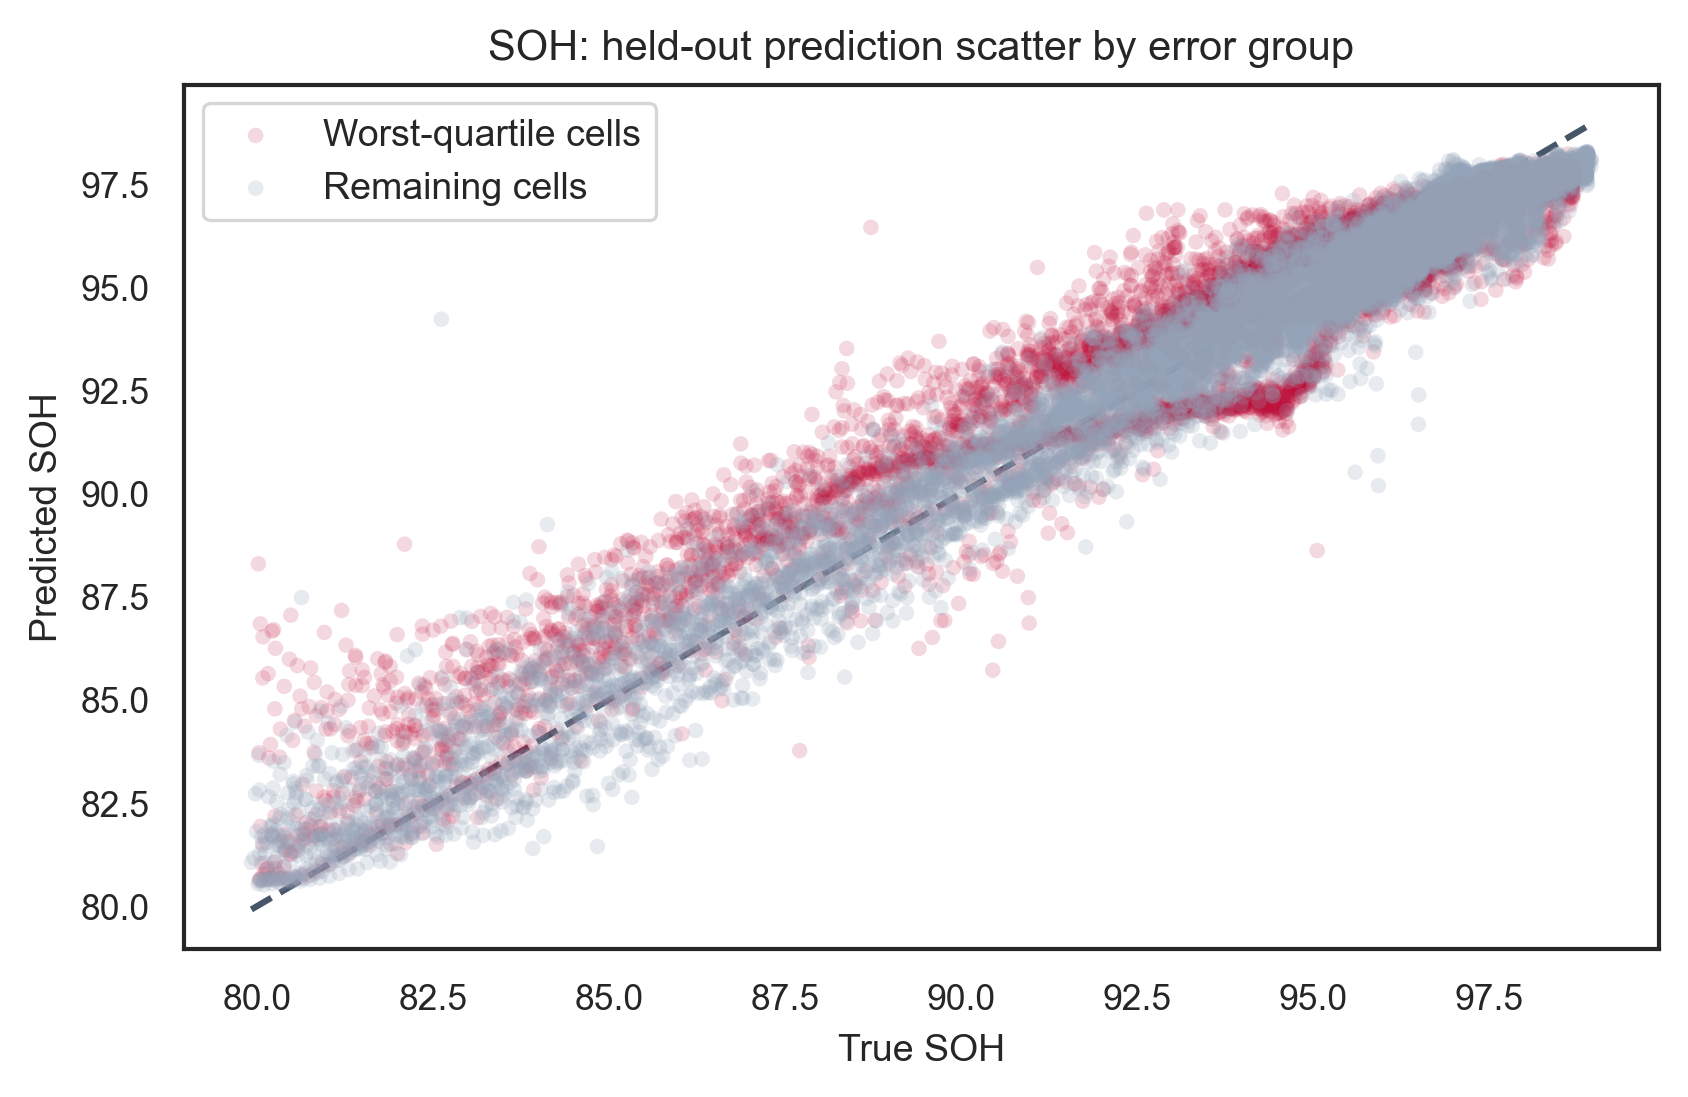
\includegraphics[width=0.8\linewidth]{../review_process/figures_revision_round1/figure_04_scatter_soh.png}
    \caption{Held-out prediction scatter for \ac{soh} highlighting whether each point belongs to the worst quartile of cells or to the remaining held-out cells according to the per-cell \ac{rmse} ranking.}
    \label{fig:diagnostics_scatter_soh}
\end{figure}

\begin{figure}[H]
    \centering
    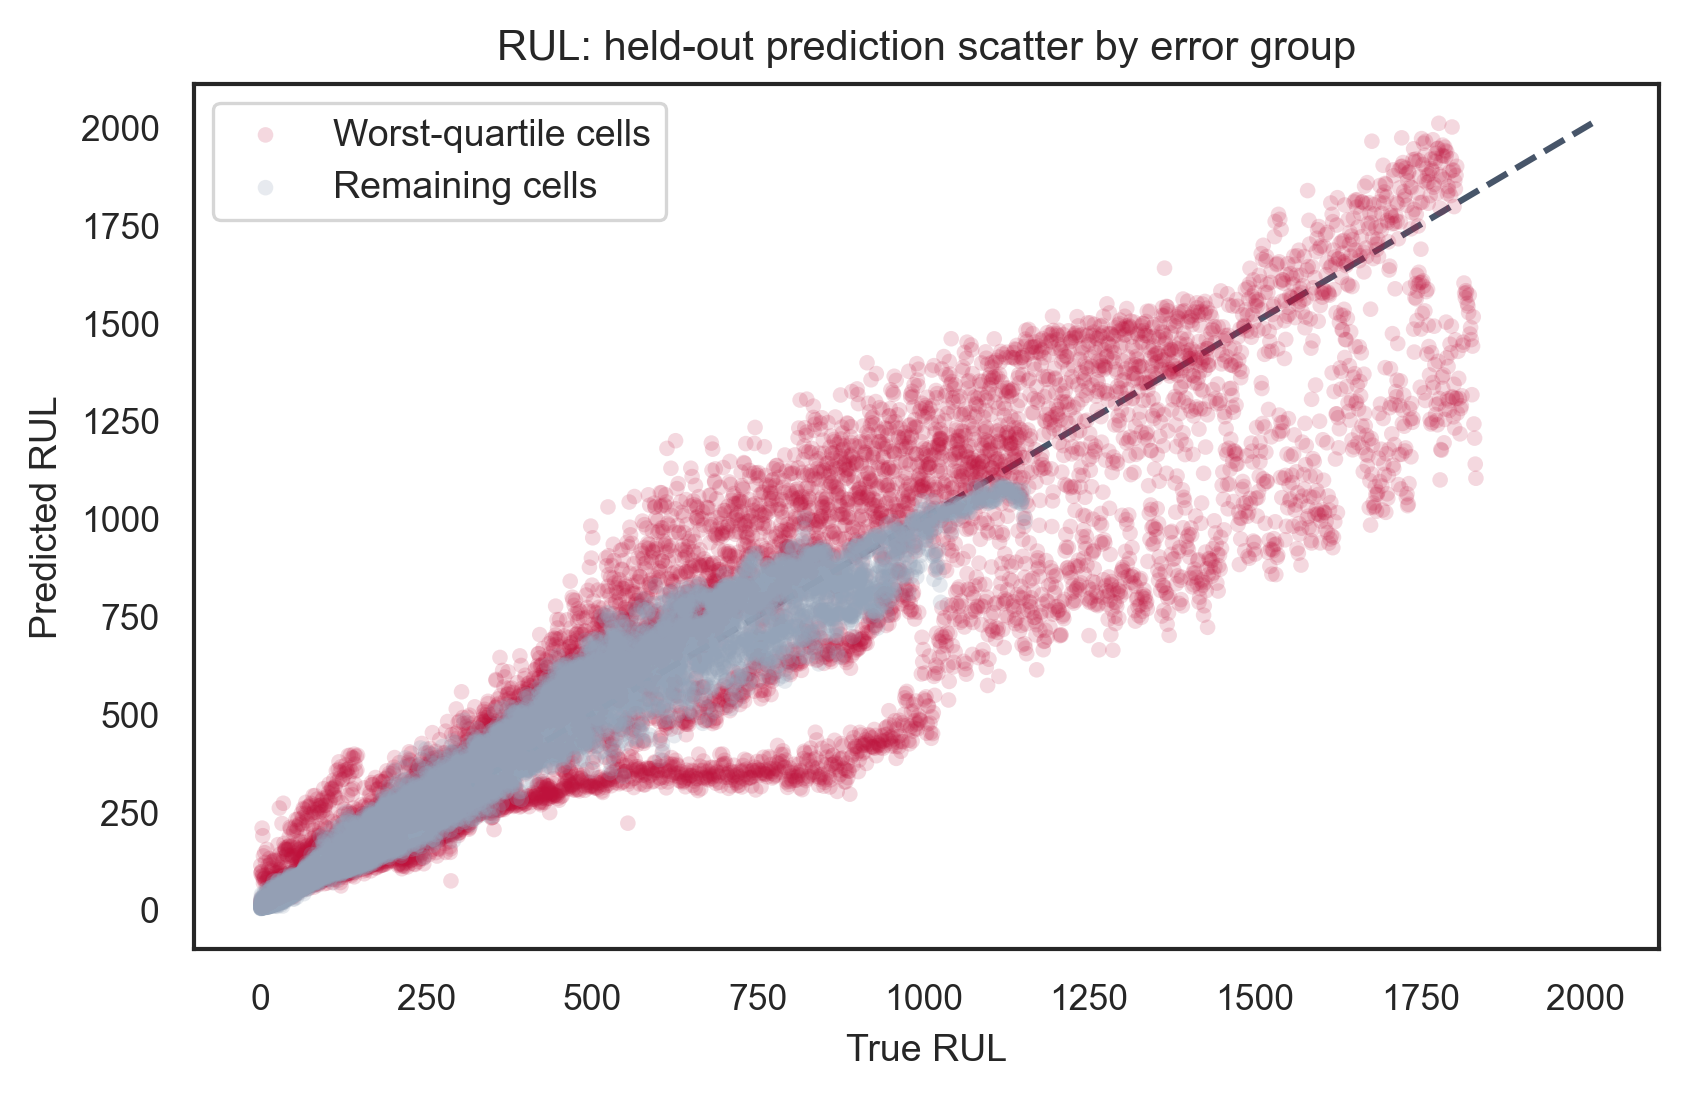
\includegraphics[width=0.8\linewidth]{../review_process/figures_revision_round1/figure_04_scatter_rul.png}
    \caption{Held-out prediction scatter for \ac{rul} highlighting whether each point belongs to the worst quartile of cells or to the remaining held-out cells according to the per-cell \ac{rmse} ranking.}
    \label{fig:diagnostics_scatter_rul}
\end{figure}

\subsection{Protocol-Family Robustness}

To test whether the learned feature-target relations generalize beyond a single random cell split, the study also evaluated leave-one-family-out robustness across protocol families defined by charging aggressiveness. Table~\cref{tab:protocol_family_robustness} summarizes these family-holdout results. In the present dataset, this yielded four non-sparse groups with exact maximum charge C-rate intervals of \([2.2116, 2.4968)\), \([2.4968, 2.7053)\), \([2.7053, 3.0411)\), and \([3.0411, 4.5878]\) C. \ac{soh} remained comparatively stable, with family-holdout \ac{rmse} between 1.2578 and 1.8110 and \(R^2\) between 0.8470 and 0.9219. \ac{rul} was more sensitive to protocol shift, ranging from 66.08 cycles for rate group 1 to 196.95 cycles for rate group 2. These results indicate that cross-cell generalization is meaningful but incomplete: the feature representation remains informative across protocol families, yet its robustness degrades when the held-out family differs more strongly in charging regime and lifetime profile.

\begin{table}[H]
    \centering
    \caption{Protocol-family robustness in the leave-one-family-out evaluation, with the confirmed maximum charge C-rate intervals used to define each group.}
    \label{tab:protocol_family_robustness}
    \resizebox{\linewidth}{!}{%
    \begin{tabular}{lrrrrrr}
    \toprule
    Rate group & Max charge C-rate interval & Mean cycle life & SOH RMSE & SOH $R^2$ & RUL RMSE & RUL $R^2$ \\
    \midrule
    0 & [2.2116, 2.4968) & 740.94 & 1.2578 & 0.9219 & 116.0194 & 0.9272 \\
    1 & [2.4968, 2.7053) & 638.94 & 1.8110 & 0.8470 & 66.0759 & 0.9158 \\
    2 & [2.7053, 3.0411) & 970.32 & 1.4331 & 0.8813 & 196.9549 & 0.7976 \\
    3 & [3.0411, 4.5878] & 847.68 & 1.4367 & 0.8840 & 175.2911 & 0.7571 \\
    \bottomrule
    \end{tabular}
    }
\end{table}


From a practical perspective, the results support lightweight prognosis from a single diagnostic cycle, but with a clearly bounded scope. \ac{soh} estimation is the stronger result, since the held-out error remains near one percentage point even with a single reference model family. \ac{rul} estimation is better interpreted as a coarse risk indicator than as a cycle-accurate forecast, especially under protocol shift or for cells with atypical trajectories. The charge-only branch remains particularly relevant for deployment, because it shows that useful prognostic structure survives even when discharge data are unavailable, although full-cycle features still provide the most stable reference point.

\subsection{Future Work}

A small set of cells appears to be underrepresented in the training population in terms of trajectory shape, protocol response, or lifetime range. Future work should therefore investigate targeted data augmentation, broader protocol coverage, or hybrid modeling strategies that improve robustness specifically in these low-support regions of the battery-lifetime space.
